\documentclass[12pt,a4paper]{report}

% ----------------------------------------------------------
% PACKAGES
% ----------------------------------------------------------
\usepackage[utf8]{inputenc}
\usepackage[french]{babel}
\usepackage[T1]{fontenc}
\usepackage{geometry}
\usepackage{graphicx}
\graphicspath{{./}{../conception/}{conception/}{Rapport/}}
\usepackage{amssymb}
\setlength{\headheight}{15pt}
\DeclareUnicodeCharacter{2713}{}
\DeclareUnicodeCharacter{2192}{$\rightarrow$}
\DeclareUnicodeCharacter{2208}{$\in$}
\usepackage{fancyhdr}
\usepackage{titlesec}
\usepackage{hyperref}
\usepackage{listings}
\usepackage{xcolor}
\usepackage{tocloft}
\usepackage{setspace}
\usepackage{float}
\usepackage{enumitem}
\usepackage{array}
\usepackage{longtable}
\usepackage{multirow}
\usepackage{booktabs}
\usepackage{caption}
\usepackage{tikz}
\usetikzlibrary{positioning,arrows.meta,shapes.geometric,fit}
\usepackage{pgfplots}
\pgfplotsset{compat=1.18}

\tikzset{
    sprintactor/.style={draw, rounded corners=2pt, align=center, minimum width=2.6cm, minimum height=0.9cm, fill=gray!8},
    sprintcase/.style={draw, ellipse, align=center, minimum width=3.3cm, minimum height=0.9cm, fill=blue!4},
    sprintclass/.style={draw, rectangle, align=left, font=\scriptsize, text width=3.8cm, fill=gray!4},
    sprintseq/.style={draw, rectangle, align=center, minimum width=2.6cm, minimum height=0.8cm, fill=gray!6},
    sprintarrow/.style={draw, -{Stealth[length=2mm]}, thick},
    sprintline/.style={draw, thick},
    sprintboundary/.style={draw, dashed, rounded corners=3pt, inner sep=0.35cm},
    sprintstart/.style={draw, circle, fill=black, minimum size=0.22cm, inner sep=0pt},
    sprintend/.style={draw, circle, minimum size=0.35cm, inner sep=0pt, path picture={
        \fill (path picture bounding box.center) circle (0.11cm);
    }},
    sprintactivity/.style={draw, rounded corners=8pt, align=center, minimum width=4.6cm, minimum height=0.9cm, fill=green!5},
    sprintdecision/.style={draw, diamond, aspect=2.1, align=center, inner sep=1pt, fill=yellow!8}
}

% ----------------------------------------------------------
% CONFIGURATION DE LA PAGE
% ----------------------------------------------------------
\geometry{
    a4paper,
    left=2cm,
    right=2cm,
    top=2.5cm,
    bottom=2.5cm
}

% ----------------------------------------------------------
% EN-TÊTE ET PIED DE PAGE
% ----------------------------------------------------------
\pagestyle{fancy}
\fancyhf{}
\fancyhead[L]{\leftmark}
\fancyhead[R]{\thepage}
\fancyfoot[C]{Institut Supérieur des Sciences Appliquées et de Technologie - Sousse}
\renewcommand{\headrulewidth}{0.5pt}
\renewcommand{\footrulewidth}{0.5pt}

% ----------------------------------------------------------
% CONFIGURATION DES TITRES
% ----------------------------------------------------------
\titleformat{\chapter}[display]
  {\normalfont\huge\bfseries}{\chaptertitlename\ \thechapter}{20pt}{\Huge}
\titlespacing*{\chapter}{0pt}{-20pt}{40pt}

% ----------------------------------------------------------
% CONFIGURATION DES LISTINGS (CODE)
% ----------------------------------------------------------
\lstset{
    basicstyle=\ttfamily\footnotesize,
    breaklines=true,
    frame=single,
    numbers=left,
    numberstyle=\tiny\color{gray},
    keywordstyle=\color{blue},
    commentstyle=\color{green!50!black},
    stringstyle=\color{red},
    backgroundcolor=\color{gray!10},
    showstringspaces=false,
    tabsize=2
}

% ----------------------------------------------------------
% HYPERLINKS
% ----------------------------------------------------------
\hypersetup{
    colorlinks=true,
    linkcolor=black,
    filecolor=magenta,
    urlcolor=blue,
    citecolor=black
}

% ----------------------------------------------------------
% DÉBUT DU DOCUMENT
% ----------------------------------------------------------
\begin{document}

% ----------------------------------------------------------
% PAGE DE GARDE
% ----------------------------------------------------------
\begin{titlepage}
    \centering
    
    \begin{minipage}[t]{0.45\textwidth}
        \raggedright
        \footnotesize
        \textbf{République Tunisienne}\\
        \textbf{Ministère de l'Enseignement}\\
        \textbf{Supérieur et de la Recherche}\\
        \textbf{Scientifique}\\
        \textbf{Université de Sousse}
        \vspace{0.8cm}
        \centering
         
\includegraphics[width=3.5cm]{Logo-Uso.jpg}
    \end{minipage}%
    \hfill
    \begin{minipage}[t]{0.45\textwidth}
        \raggedleft
        \footnotesize
        \textbf{Institut Supérieur des}\\
        \textbf{Sciences Appliquées et}\\
        \textbf{de Technologie de Sousse}\\
        \vspace{1cm}
        \centering
        
\includegraphics[width=4.5cm]{issat.png}
    \end{minipage}
    
    \vspace{2cm}
    
    {\large \textbf{Département Informatique}}
    
    \vspace{2.5cm}
    
    {\Large \textbf{\textit{RAPPORT DE MINI PROJET}}}\\[0.8cm]
    {\Large \textbf{\textit{Développement Web}}}\\[0.5cm]
    {\large \textbf{\textit{ING-A2-GL}}}
    
    \vspace{2cm}
    
    {\Huge \textbf{\textit{Application Web de Gestion}}}\\[0.5cm]
    {\Huge \textbf{\textit{d'Institut Universitaire}}}\\[0.3cm]
    
    \vfill
    
    \begin{flushleft}
        \hspace{1.5cm}
        \textbf{Préparé par :}\\[0.3cm]
        \hspace{3cm} Fourat Jebali\\
        \hspace{3cm} Mohamed Amin Neji
    \end{flushleft}
    
    \vspace{1cm}
    
    \textbf{Année Universitaire : 2025 / 2026}
\end{titlepage}

% ----------------------------------------------------------
% TABLE DES MATIÈRES
% ----------------------------------------------------------
\tableofcontents
\newpage

% ----------------------------------------------------------
% LISTE DES FIGURES
% ----------------------------------------------------------
\listoffigures
\newpage

% ----------------------------------------------------------
% LISTE DES TABLEAUX
% ----------------------------------------------------------
\listoftables
\newpage
\chapter*{Introduction générale}
\addcontentsline{toc}{chapter}{Introduction générale}

Dans le contexte actuel de transformation numérique de l'enseignement supérieur, les instituts universitaires doivent gérer un volume croissant d'informations administratives et pédagogiques. La multiplicité des acteurs impliqués, tels que les étudiants, les professeurs et les administrateurs, ainsi que la diversité des procédures à traiter, rendent la gestion manuelle de plus en plus complexe et peu efficace.

En effet, l'utilisation d'outils dispersés, de traitements manuels et de supports non centralisés peut engendrer des pertes de temps, des erreurs, un manque de traçabilité et des difficultés d'accès à l'information. Face à ces limites, la mise en place d'une solution informatique intégrée apparaît comme une nécessité pour améliorer l'organisation, la fiabilité et la fluidité des processus académiques.

C'est dans cette optique que s'inscrit notre projet, qui consiste à concevoir et développer une application web de gestion d'institut universitaire. Cette application a pour finalité d'automatiser et de centraliser les principales procédures liées à la gestion des utilisateurs, de la structure pédagogique, des notes, des présences, des annonces, des emplois du temps, des examens et des supports de cours.

Le présent rapport décrit la démarche adoptée pour la réalisation de ce projet. Il présente d'abord le contexte général, les besoins identifiés et les choix méthodologiques retenus. Il détaille ensuite l'analyse, la conception, la réalisation technique et enfin les résultats obtenus à travers les tests et l'évaluation de la solution proposée.

\newpage

% ==========================================================
% CHAPITRE 1 : GÉNÉRALISATION
% ==========================================================
\chapter{Généralisation}

\section{Introduction du chapitre}

Ce chapitre présente le cadre général du projet de gestion d'institut universitaire. Il expose d'abord le contexte dans lequel s'inscrit ce travail, ainsi que la problématique à laquelle il répond. Ensuite, il précise les objectifs visés et le périmètre fonctionnel de l'application. Enfin, il décrit les choix méthodologiques et techniques adoptés pour mener à bien le développement de la solution.


\section{Contexte du Projet}

\subsection{Problématique}

Les instituts universitaires traitent quotidiennement un grand nombre d'informations qui sont réparties sur différents sites et personnes. Cette dispersion crée divers problèmes :

\begin{itemize}[itemsep=0.5em]
    \item \textbf{Manque de centralisation} : les informations sont dispersées entre des fichiers Excel, du paperwork, ou même des bases de données qui ne sont pas interconnectées ;
    \item \textbf{Des procédures manuelles} : les saisies de notes, l'assiduité, l'affichage de l'information requièrent une procédure manuelle qui consomme du temps ;
    \item \textbf{Accès difficile aux informations} : Les étudiants et professeurs peinent à obtenir rapidement les informations dont ils ont besoin
    \item \textbf{Risques d'erreurs} : La manipulation manuelle des données augmente les risques d'incohérences et d'erreurs
    \item \textbf{Absence de traçabilité} : impossible de connaître toute l'histoire de la base de données
\end{itemize}

\subsection{Objectifs du Projet}

L'objectif principal de ce projet est de développer une application web complète permettant de :

\begin{enumerate}[itemsep=0.5em]
    \item \textbf{Centraliser la gestion académique} dans une plateforme unique et cohérente
    \item \textbf{Automatiser les processus répétitifs} (calcul de moyennes, notifications, validation de données)
    \item \textbf{Faciliter la communication} entre les différents acteurs de l'institut
    \item \textbf{Améliorer la traçabilité} grâce à un système d'historisation et de logs
    \item \textbf{Sécuriser l'accès aux données} par un système d'authentification et d'autorisation basé sur les rôles
    \item \textbf{Offrir une interface intuitive} adaptée aux besoins de chaque type d'utilisateur
\end{enumerate}

\subsection{Périmètre Fonctionnel}

L'application couvre les modules suivants :

\begin{table}[H]
\centering
\caption{Modules fonctionnels de l'application}
\begin{tabular}{|p{4cm}|p{10cm}|}
\hline
\textbf{Module} & \textbf{Description} \\
\hline
Authentification & Gestion sécurisée des connexions avec JWT et gestion des rôles (Étudiant, Professeur, Administrateur) \\
\hline
Structure Pédagogique & Gestion des départements, matières, groupes et enseignements \\
\hline
Utilisateurs & Gestion des profils étudiants, professeurs et administrateurs \\
\hline
Notes \& Évaluations & Saisie, validation et publication des notes avec calcul automatique des moyennes \\
\hline
Présences \& Rattrapages & Gestion des présences/absences et organisation des séances de rattrapage \\
\hline
Annonces & Publication et consultation d'annonces ciblées par groupe ou globales \\
\hline
Emplois du Temps & Planification et consultation des séances avec détection de conflits horaires \\
\hline
Supports de Cours & Upload, stockage et téléchargement de documents pédagogiques \\
\hline
\end{tabular}
\end{table}

\section{Choix Méthodologiques}

\subsection{Processus de Développement : Scrum Allégé Hybride}

Pour réaliser notre projet, nous avons mis en place une méthodologie appelée \textbf{Scrum Allégé Hybride}, qui est adaptée à l'environnement de travail d'une équipe de deux personnes. Cette méthode combine les points positifs du Scrum avec la souplesse requise pour une telle petite équipe.

\subsubsection{Justification du Choix}

\begin{enumerate}[itemsep=0.5em]
    \item \textbf{Adaptabilité pour binôme} : Cadre structurel suffisant pour assurer la discipline sans le surcroît d'administratif inhérent aux grosses équipes.
    \item \textbf{Coordination efficace} : assure une coordination permanente entre une équipe de deux personnes.
    \item \textbf{Architecture modulaire} : 8 modules définis qui s'y prêteraient très bien pour un développement incrémental avec livraison incrémentale de fonctionnalités.
    \item \textbf{Complexité maîtrisée} : Plus de 15 entités ayant des relations complexes, nécessitent une approche progressive.
\end{enumerate}

% ---- [AJOUT SCRUM] Définition des rôles de l'équipe ----
\subsubsection{Rôles Scrum dans l'Équipe}

Dans le cadre de notre Scrum allégé hybride adapté à un binôme, les rôles Scrum ont été définis comme suit :

\begin{table}[H]
\centering
\caption{Répartition des rôles Scrum au sein du binôme}
\begin{tabular}{|p{4cm}|p{4cm}|p{6cm}|}
\hline
\textbf{Rôle Scrum} & \textbf{Assigné à} & \textbf{Responsabilités} \\
\hline
\textbf{Product Owner} & Fourat Jebali & Définit et priorise le Product Backlog, valide les critères d'acceptation, représente les besoins fonctionnels \\
\hline
\textbf{Scrum Master} & Mohamed Amin Neji & Facilite les cérémonies Scrum, lève les obstacles techniques, veille au respect du cadre méthodologique \\
\hline
\textbf{Équipe de Développement} & Fourat Jebali \& Mohamed Amin Neji & Développement backend (PA) et frontend (PB), tests, documentation \\
\hline
\end{tabular}
\end{table}

\textit{Note : Dans un binôme, le Product Owner et le Scrum Master endossent également des rôles de développement. Ce double rôle est une adaptation validée du Scrum pour les petites équipes.}

\subsubsection{Organisation en Sprints}

Le projet est organisé en \textbf{sept sprints} : un sprint d'initialisation technique, quatre sprints fonctionnels alignés sur les modules principaux, un sprint de stabilisation et de validation, puis un sprint d'amélioration UI/UX destiné à renforcer l'expérience utilisateur avant la soutenance.

\begin{table}[H]
\centering
\caption{Planning des sprints}
\begin{tabular}{|c|p{3cm}|p{8cm}|c|}
\hline
\textbf{Sprint} & \textbf{Durée} & \textbf{Objectifs Principaux} & \textbf{Story Points} \\
\hline
Sprint 0 & 1 semaine & Setup infrastructure, Docker, projets Spring Boot et Angular & 13 \\
\hline
Sprint 1 & 2 semaines & Module authentification : API JWT, refresh token, stockage frontend, guards et redirection par rôle & 35 \\
\hline
Sprint 2 & 2 semaines & Module administrateur : dashboard, structure académique, années/semestres, examens, validation des notes et supervision des présences & 35 \\
\hline
Sprint 3 & 2 semaines & Module professeur : dashboard, enseignements, séances, évaluations, notes, appel de présence optimisé, rattrapages et supports de cours & 40 \\
\hline
Sprint 4 & 2 semaines & Module étudiant : annonces par défaut, notifications, notes publiées, emploi du temps, calendrier des examens, supports, rattrapages et suivi des absences & 36 \\
\hline
Sprint 5 & 1 semaine & Tests, validation globale, corrections finales et finalisation documentaire & 20 \\
\hline
Sprint 6 & 1 semaine & Améliorations UI/UX : thème clair/sombre, sidebar masquable, centre de notifications, calendrier académique, pagination et ergonomie des examens & 34 \\
\hline
\end{tabular}
\end{table}

% ---- [AJOUT SCRUM] Definition of Done globale ----
\subsubsection{Définition of Done (DoD) Globale}

La \textbf{Definition of Done} définit les critères qu'une User Story doit satisfaire pour être considérée comme terminée. Elle s'applique à l'ensemble des sprints du projet :

\begin{itemize}[itemsep=0.4em]
    \item  Le code source est versionné sur GitHub dans la branche appropriée (feature branch mergée dans \texttt{dev})
    \item  Les tests unitaires associés sont écrits et passent avec succès (couverture $\geq$ 75\%)
    \item  Le code a été relu par l'autre membre de l'équipe (code review)
    \item  La fonctionnalité est intégrée et testée dans l'environnement Docker Compose
    \item  Les critères d'acceptation de la User Story sont tous vérifiés manuellement
    \item  La documentation technique (JavaDoc / commentaires Angular) est à jour
    \item  Aucune régression introduite sur les fonctionnalités existantes
\end{itemize}

\subsection{Stack Technique}

Le choix de la stack technique a été guidé par les critères suivants : maturité des technologies, richesse de l'écosystème, facilité de déploiement et compétences de l'équipe.

\begin{table}[H]
\centering
\caption{Stack technique du projet}
\begin{tabular}{|p{3cm}|p{4cm}|p{7cm}|}
\hline
\textbf{Couche} & \textbf{Technologie} & \textbf{Justification} \\
\hline
Frontend & Angular 17+ & Framework mature, TypeScript typé, Angular Material pour UI \\
\hline
Backend & Spring Boot 3.x & Écosystème Java robuste, Spring Security pour l'authentification, Spring Data JPA pour l'ORM \\
\hline
Base de Données & PostgreSQL 14+ & SGBD relationnel performant, support complet des contraintes d'intégrité \\
\hline
Authentification & JWT (jsonwebtoken) & Standard industry pour authentification stateless, facile à implémenter \\
\hline
Migrations DB & Flyway & Gestion versionnée du schéma de base de données \\
\hline
Containerisation & Docker \& Docker Compose & Environnements reproductibles, facilite le déploiement \\
\hline
CI/CD & GitHub Actions & Intégration native avec GitHub, pipelines simples à configurer \\
\hline
Reverse Proxy & NGINX & Performant, gestion SSL/TLS, load balancing \\
\hline
\end{tabular}
\end{table}

\subsection{Architecture Applicative}

L'application suit une \textbf{architecture 3-tiers} classique :

\begin{enumerate}[itemsep=0.5em]
    \item \textbf{Couche Présentation (Frontend)} : Application Angular SPA (Single Page Application) communiquant avec le backend via API REST
    \item \textbf{Couche Métier (Backend)} : Spring Boot exposant des endpoints REST, implémentant la logique métier et gérant la sécurité
    \item \textbf{Couche Données} : PostgreSQL stockant l'ensemble des données avec contraintes d'intégrité référentielle
\end{enumerate}

Cette séparation claire des responsabilités permet :
\begin{itemize}
    \item Une maintenance facilitée
    \item Une scalabilité horizontale (ajout de serveurs backend)
    \item Une testabilité accrue (tests unitaires par couche)
    \item Une réutilisabilité potentielle (l'API peut servir d'autres clients)
\end{itemize}

\section{Analyse des Besoins}

\subsection{Acteurs du Système}

Le système identifie trois types d'acteurs principaux ayant des rôles et des privilèges distincts :

\begin{table}[H]
\centering
\caption{Acteurs du système et leurs responsabilités}
\begin{tabular}{|p{3cm}|p{11cm}|}
\hline
\textbf{Acteur} & \textbf{Responsabilités Principales} \\
\hline
\textbf{Étudiant} & 
\begin{itemize}[leftmargin=*, nosep]
    \item Consulter ses notes publiées et moyennes
    \item Consulter son emploi du temps
    \item Télécharger les supports de cours
    \item Consulter les annonces publiées dès l'accès à l'espace étudiant
    \item Consulter les notifications importantes (annonces, notes, rattrapages, examens)
    \item Consulter les rattrapages programmés
    \item Consulter le calendrier des examens publiés
    \item Suivre ses absences et les risques d'élimination
\end{itemize} \\
\hline
\textbf{Professeur} & 
\begin{itemize}[leftmargin=*, nosep]
    \item Créer, modifier et supprimer ses évaluations
    \item Saisir et modifier les notes des étudiants
    \item Réaliser l'appel avec marquage rapide Présent/Absent
    \item Créer et gérer les séances de rattrapage
    \item Déposer des supports de cours
    \item Consulter les groupes assignés
    \item Consulter l'emploi du temps des enseignements
\end{itemize} \\
\hline
\textbf{Administrateur} & 
\begin{itemize}[leftmargin=*, nosep]
    \item Gérer les utilisateurs (création, modification, suppression)
    \item Gérer la structure pédagogique (départements, matières, groupes)
    \item Créer et planifier les enseignements
    \item Gérer le calendrier des examens
    \item Publier les annonces
    \item Publier les notes après délibération
    \item Contrôler et valider les notes saisies par les professeurs
\end{itemize} \\
\hline
\end{tabular}
\end{table}

\subsection{Besoins Fonctionnelles Principales}

\begin{enumerate}[itemsep=0.5em]
    \item \textbf{Authentification et Autorisation}
    \begin{itemize}
        \item Connexion sécurisée via email et mot de passe
        \item Génération de tokens JWT avec expiration
        \item Contrôle d'accès basé sur les rôles (RBAC)
        \item Refresh token pour maintenir la session
    \end{itemize}
    
    \item \textbf{Gestion de la Structure Pédagogique}
    \begin{itemize}
        \item CRUD complet pour départements, matières, groupes
        \item Association many-to-many départements-matières
        \item Création d'enseignements avec semestre et année universitaire
        \item Validation de l'unicité des codes matières
    \end{itemize}
    
    \item \textbf{Gestion des Notes}
    \begin{itemize}
        \item Création et gestion des évaluations par le professeur avant la saisie des notes
        \item Saisie batch des notes par le professeur
        \item Validation automatique (notes entre 0 et 20)
        \item Workflow de validation (Brouillon → Validée Prof → Validée Admin → Publiée)
        \item Calcul automatique des moyennes pondérées
        \item Notification des étudiants lors de la publication
    \end{itemize}
    
    \item \textbf{Gestion des Présences}
    \begin{itemize}
        \item Prise de présence par séance avec statuts (Présent, Absent)
        \item Marquage rapide des absents avec tous les étudiants présents par défaut
        \item Statistiques de présence par étudiant
        \item Identification des étudiants en situation d'absence excessive
    \end{itemize}
\end{enumerate}

\subsection{Besoins Non-Fonctionnelles}

\begin{table}[H]
\centering
\caption{Exigences non-fonctionnelles}
\begin{tabular}{|p{3.5cm}|p{10cm}|}
\hline
\textbf{Catégorie} & \textbf{Exigences} \\
\hline
\textbf{Performance} & 
\begin{itemize}[leftmargin=*, nosep]
    \item Temps de réponse API < 2 secondes pour 95\% des requêtes
    \item Support de 100 utilisateurs simultanés
    \item Pagination pour les listes volumineuses
\end{itemize} \\
\hline
\textbf{Sécurité} & 
\begin{itemize}[leftmargin=*, nosep]
    \item Mots de passe hashés avec BCrypt
    \item Tokens JWT expirables et renouvelables
    \item HTTPS obligatoire en production
    \item Protection CORS configurée
    \item Validation des entrées utilisateur
\end{itemize} \\
\hline
\textbf{Disponibilité} & 
\begin{itemize}[leftmargin=*, nosep]
    \item Uptime cible : 99\% en production
    \item Sauvegarde quotidienne de la base de données
    \item Logs centralisés pour diagnostic
\end{itemize} \\
\hline
\textbf{Maintenabilité} & 
\begin{itemize}[leftmargin=*, nosep]
    \item Code documenté (JavaDoc, JSDoc)
    \item Tests unitaires avec couverture > 75\%
    \item Architecture modulaire et découplée
    \item Migrations DB versionnées avec Flyway
\end{itemize} \\
\hline
\textbf{Utilisabilité} & 
\begin{itemize}[leftmargin=*, nosep]
    \item Interface responsive (mobile, tablette, desktop)
    \item Accessibilité WCAG 2.1 niveau AA
    \item Feedback utilisateur pour chaque action
    \item Messages d'erreur explicites
\end{itemize} \\
\hline
\end{tabular}
\end{table}

% ==========================================================
% CHAPITRE 2 : CONCEPTION
% ==========================================================
\chapter{Conception}

\section{Introduction du chapitre}

La phase de conception constitue une étape cruciale dans le développement de notre application. Elle permet de modéliser le système avant l'implémentation, d'identifier les entités métier, de définir les interactions entre les acteurs et le système, et de spécifier les comportements attendus.

Cette conception s'appuie sur les diagrammes UML standards (cas d'utilisation, classes, séquence, activité, composants, déploiement) pour garantir une compréhension partagée entre les membres de l'équipe et assurer la cohérence de l'architecture.

\section{Diagrammes de Conception}

\subsection{Diagramme de Cas d'Utilisation}

Le diagramme de cas d'utilisation (Figure \ref{fig:usecase}) présente l'ensemble des fonctionnalités accessibles par chaque type d'acteur. On constate une séparation claire des privilèges :

\begin{itemize}[itemsep=0.5em]
    \item Les \textbf{étudiants} ont un accès en lecture seule aux informations les concernant
    \item Les \textbf{professeurs} peuvent saisir et gérer les données pédagogiques de leurs enseignements
    \item Les \textbf{administrateurs} ont un contrôle total sur la configuration et la validation des données
\end{itemize}

\textit{Note : Toutes les fonctionnalités métier nécessitent une authentification préalable (précondition générale).}

\begin{figure}[H]
    \centering
    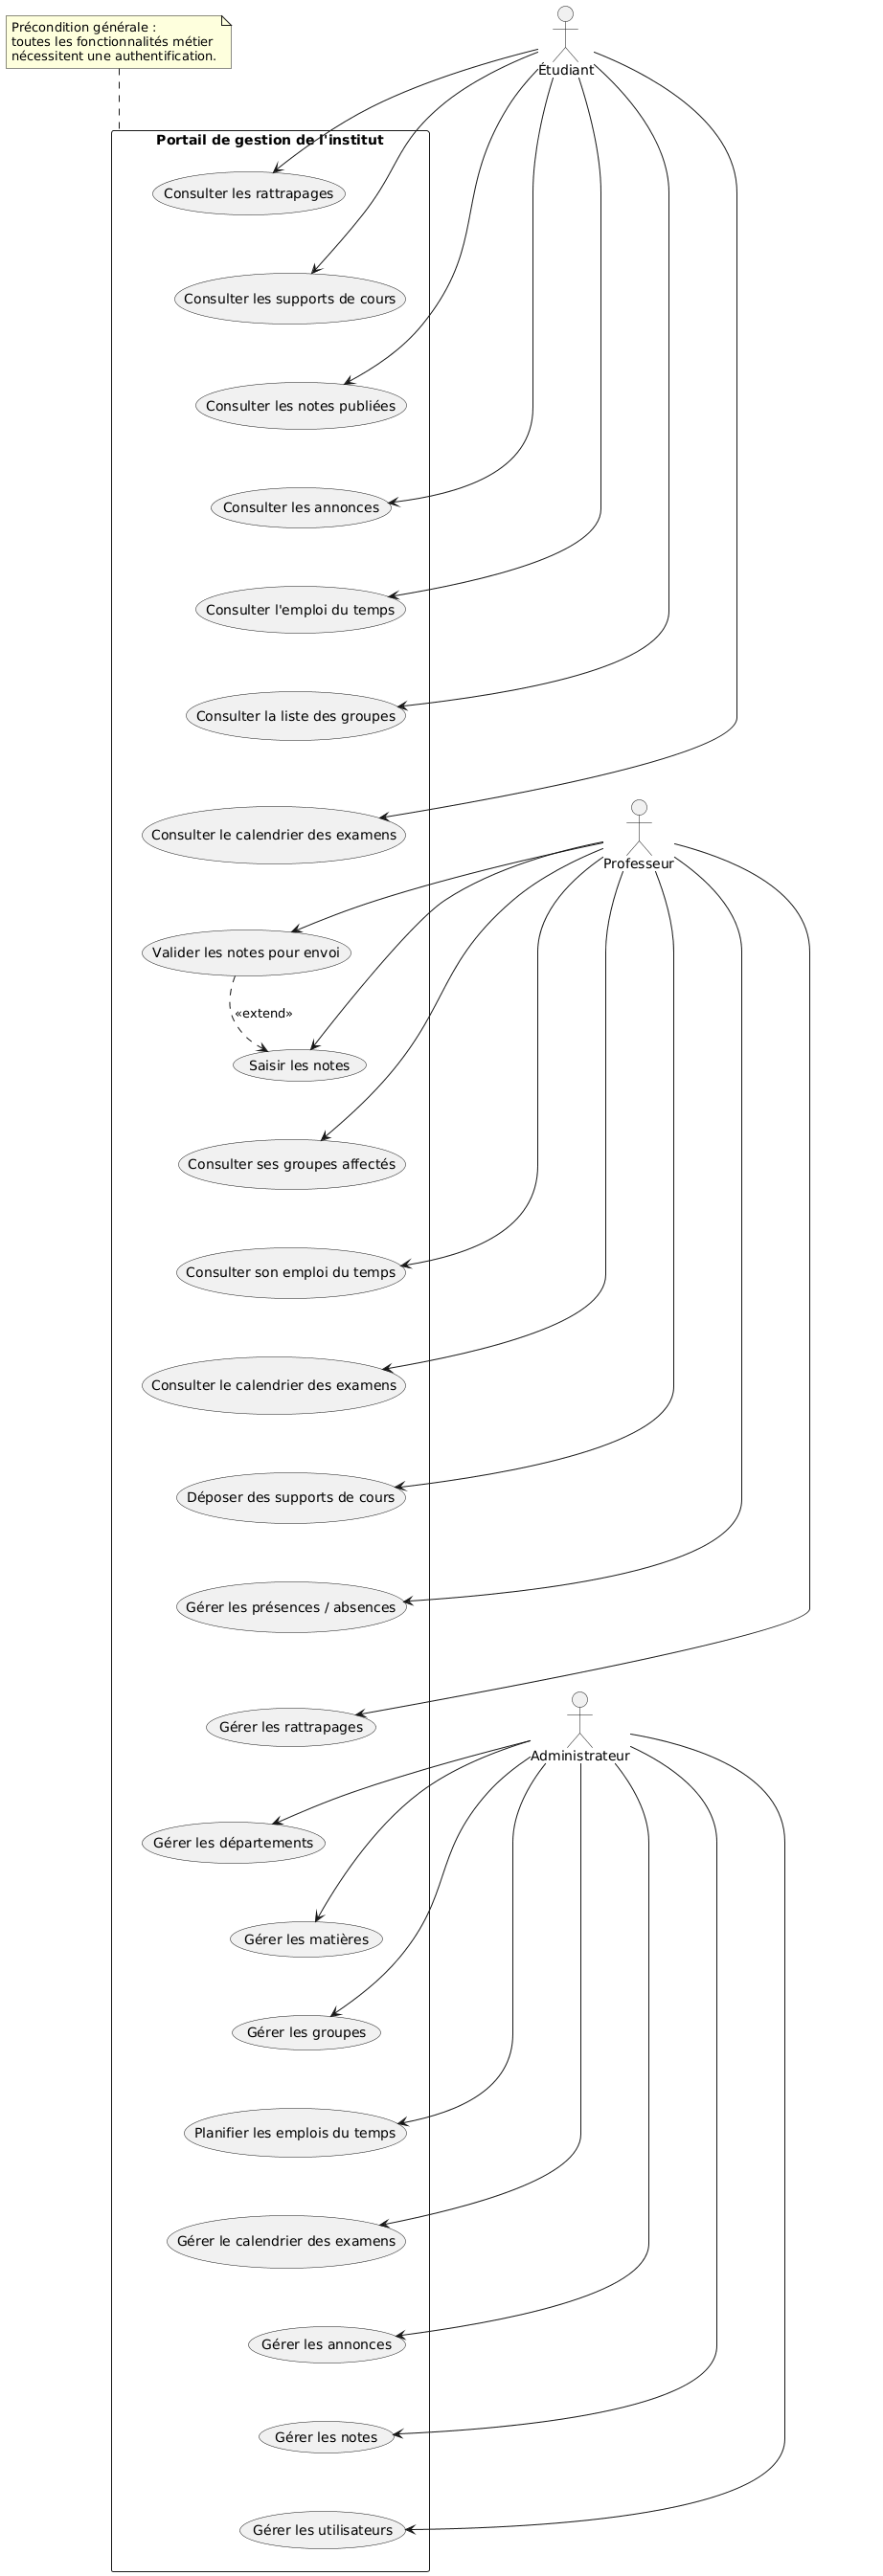
\includegraphics[width=5cm]{useCase.png}
    \caption{Diagramme de cas d'utilisation}
    \label{fig:usecase}
\end{figure}

\subsection{Diagramme de Classes}

Le diagramme de classes (Figure \ref{fig:class}) constitue le cœur de la modélisation métier. Il définit :

\begin{itemize}[itemsep=0.5em]
    \item \textbf{15 entités principales} représentant les concepts métier
    \item \textbf{Héritage} : La classe \texttt{Utilisateur} est abstraite et héritée par \texttt{Etudiant}, \texttt{Professeur} et \texttt{Administrateur} (stratégie JOINED en JPA)
    \item \textbf{Relations complexes} :
    \begin{itemize}
        \item Many-to-Many : Département $\leftrightarrow$ Matière, Groupe $\leftrightarrow$ Enseignement
        \item One-to-Many : Enseignement $\rightarrow$ Évaluation, Évaluation $\rightarrow$ Note
        \item One-to-One : Étudiant $\leftrightarrow$ Groupe
    \end{itemize}
    \item \textbf{Énumérations} : \texttt{TypeSeance} (COURS, TD, TP, RATTRAPAGE), \texttt{StatutPresence}, \texttt{TypeEvaluation}, \texttt{StatutNote}
\end{itemize}

\textbf{Points clés de conception :}

\begin{enumerate}[itemsep=0.5em]
    \item \textbf{Séparation Utilisateur/Rôles} : Évite la duplication et permet une gestion unifiée des credentials
    \item \textbf{Note avec Statut} : Workflow de validation tracé (Brouillon → Validée Prof → Validée Admin → Publiée)
    \item \textbf{Enseignement comme pivot} : Relie Matière, Professeur, Groupe, Séances et Évaluations
    \item \textbf{Annonce ciblée} : Relation optionnelle avec Groupe pour annonces globales ou ciblées
\end{enumerate}

\begin{figure}[H]
    \centering
    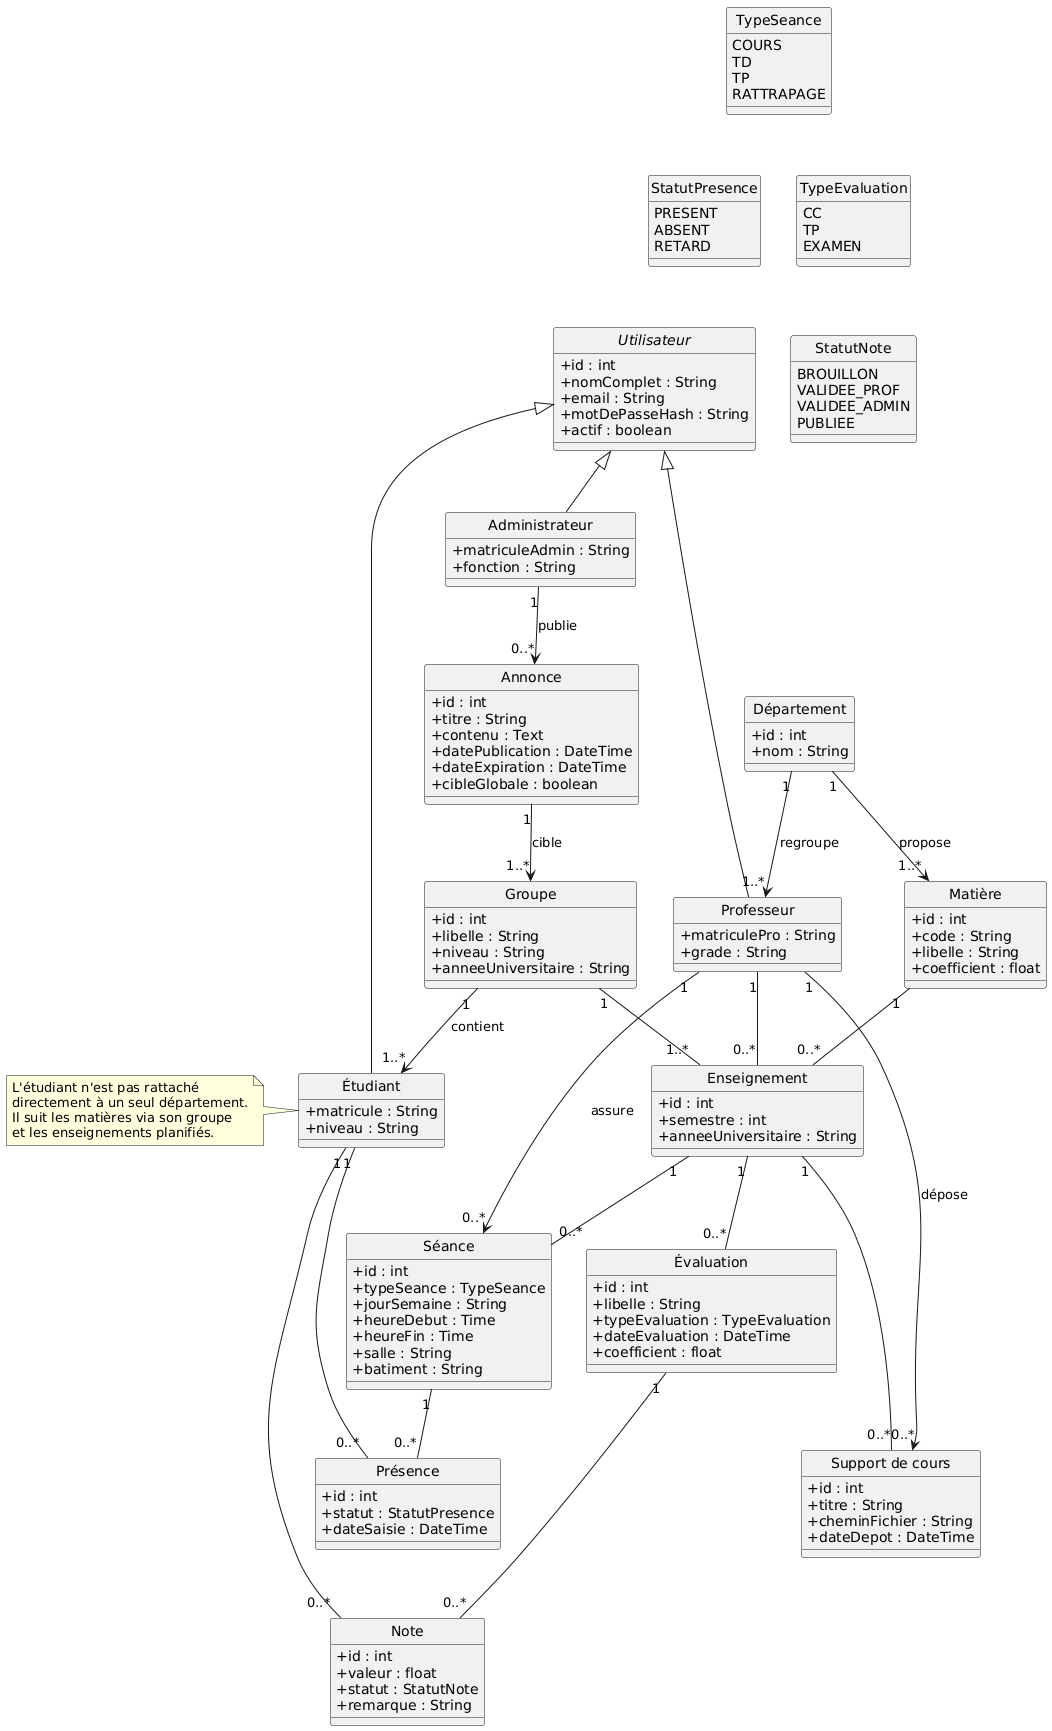
\includegraphics[width=15cm]{Class.png}
    \caption{Diagramme de classes}
    \label{fig:class}
\end{figure}

\subsection{Diagramme de Composants}

Le diagramme de composants (Figure \ref{fig:component}) illustre l'architecture modulaire de l'application web :

\begin{itemize}[itemsep=0.5em]
    \item \textbf{Interface Web} : 3 espaces distincts (Administrateur, Étudiant, Professeur)
    \item \textbf{8 modules métier} :
    \begin{enumerate}
        \item Module Structure pédagogique
        \item Module Utilisateurs
        \item Module Annonces
        \item Module Notes et délibération
        \item Module Emplois du temps
        \item Module Authentification
        \item Module Présences et rattrapages
        \item Module Supports de cours
    \end{enumerate}
    \item \textbf{Persistance} : Base de données centralisée + Stockage local des fichiers
\end{itemize}

\begin{figure}[H]
    \centering
    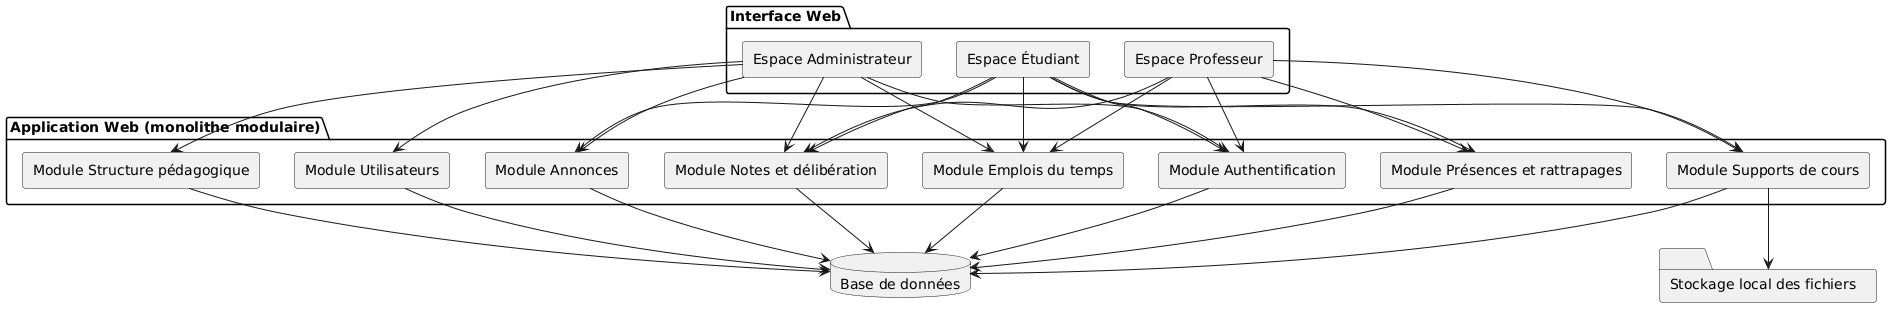
\includegraphics[width=15cm]{Component.png}
    \caption{Diagramme de composants}
    \label{fig:component}
\end{figure}

\subsection{Diagramme de Déploiement}

Le diagramme de déploiement (Figure \ref{fig:deployment}) présente l'infrastructure de production prévue :

\begin{enumerate}[itemsep=0.5em]
    \item \textbf{Client Devices} : Navigateurs Web et applications mobiles accédant via HTTPS
    \item \textbf{Load Balancer (NGINX)} : Répartition de charge et reverse proxy avec terminaison SSL/TLS
    \item \textbf{Application Servers (2 instances)} : Conteneurs Spring Boot déployés pour haute disponibilité
    \item \textbf{Database Server} : PostgreSQL primaire avec réplication asynchrone vers base secondaire
    \item \textbf{Services auxiliaires} :
    \begin{itemize}
        \item Cache Server (Redis) pour améliorer les performances
        \item File Storage Server (MinIO/S3) pour les supports de cours
        \item Email Server (SMTP) pour les notifications
    \end{itemize}
\end{enumerate}

\begin{figure}[H]
    \centering
    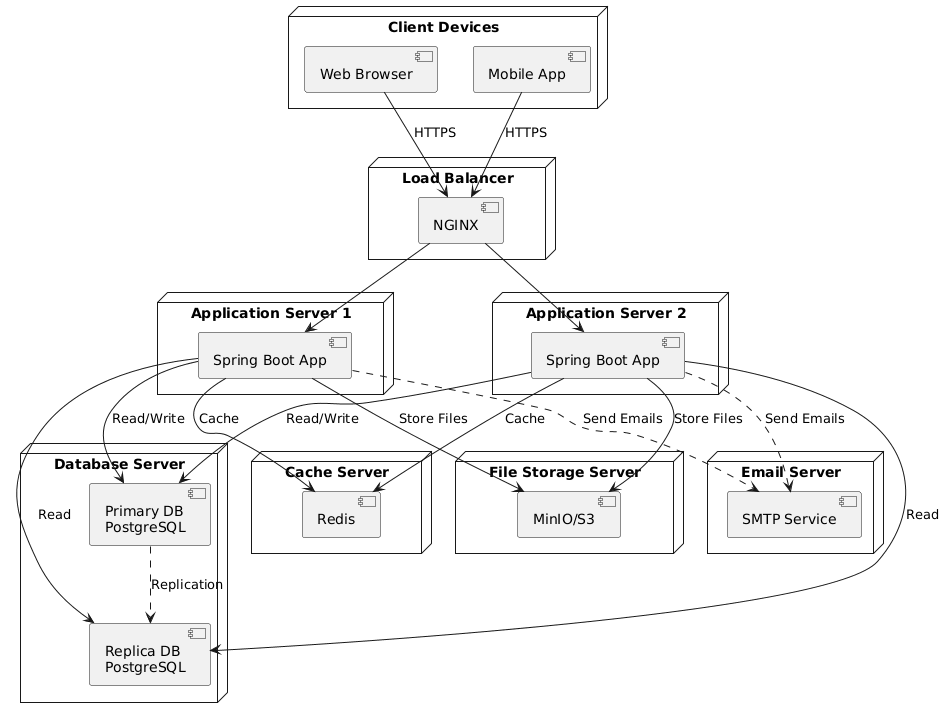
\includegraphics[width=15cm]{deployement.png}
    \caption{Diagramme de déploiement}
    \label{fig:deployment}
\end{figure}

\subsection{Diagrammes de Séquence}

\subsubsection{Séquence : Saisie de Notes par le Professeur}

\begin{figure}[H]
    \centering
    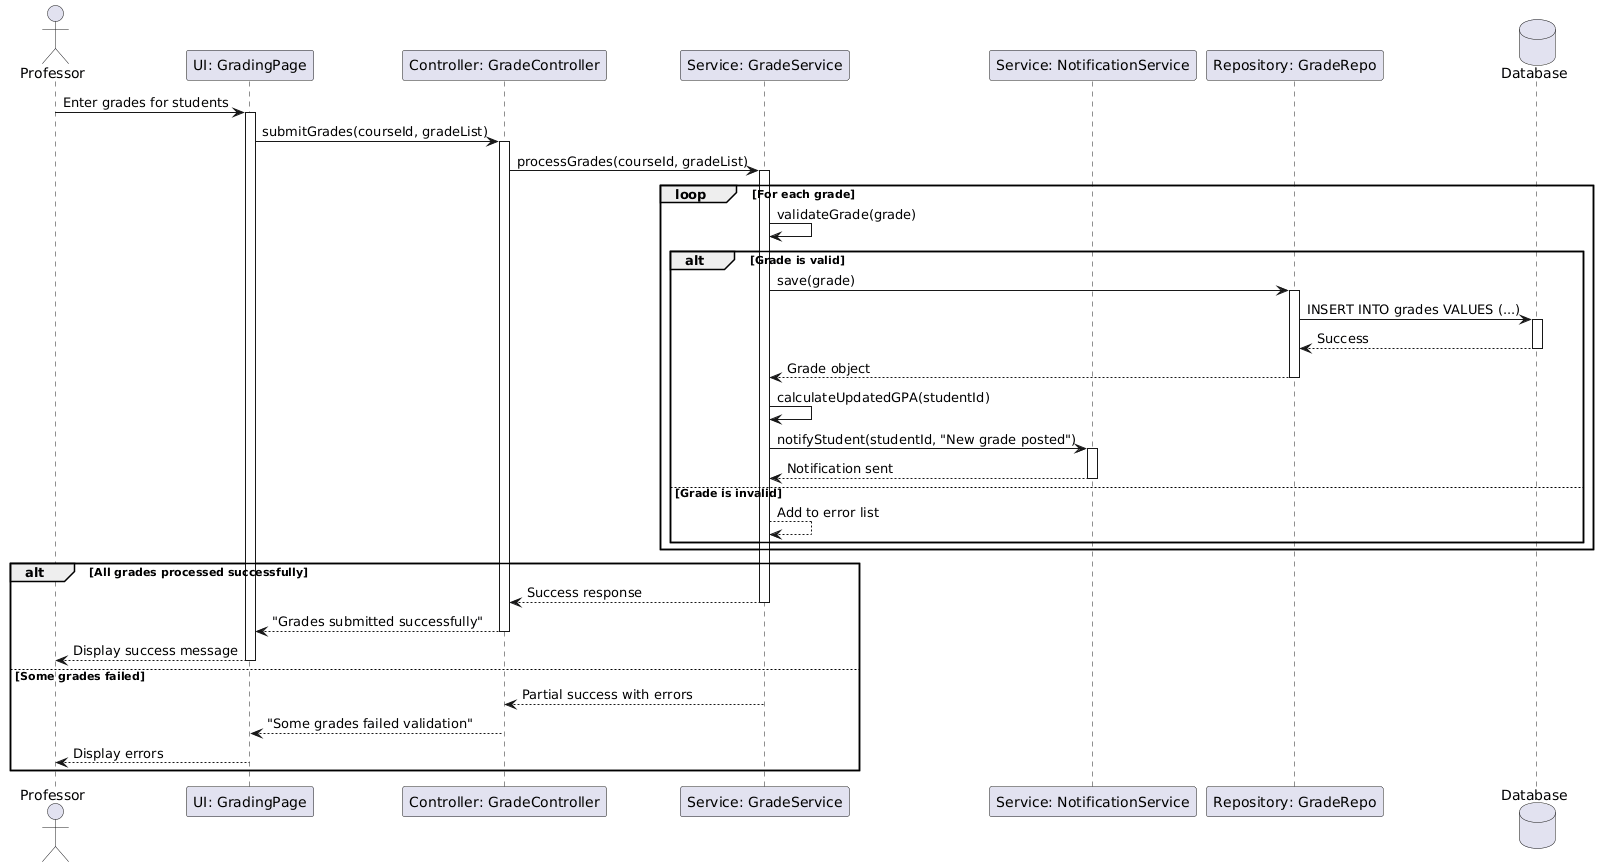
\includegraphics[width=15cm]{SEQUENCE DIAGRAM - Professor Grade Entry.png}
    \caption{Diagramme de séquence : Saisie de notes par le professeur}
    \label{fig:seq-grade}
\end{figure}

\subsubsection{Séquence : Inscription d'un Étudiant à un Cours}

\begin{figure}[H]
    \centering
    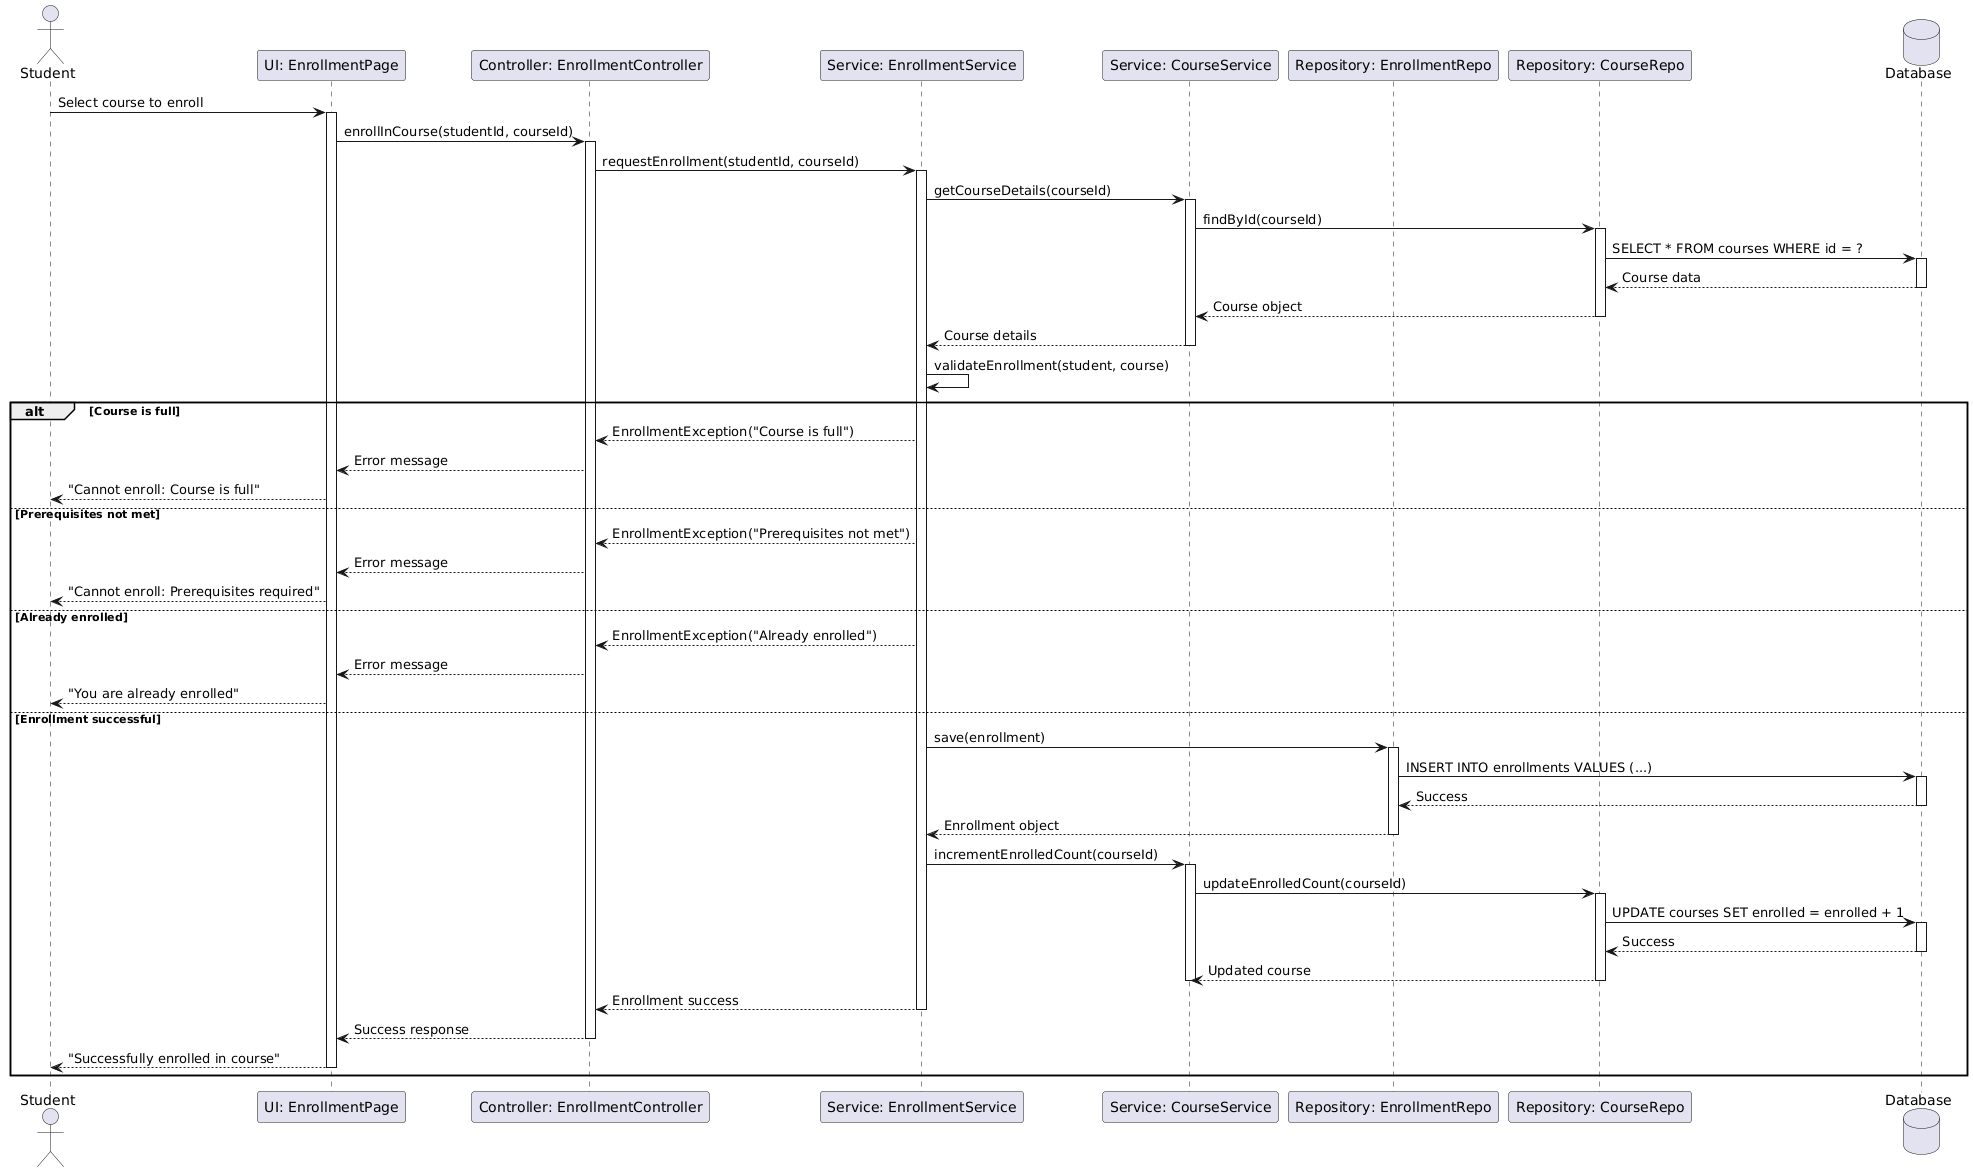
\includegraphics[width=15cm]{Sequence.png}
    \caption{Diagramme de séquence : Inscription d'un étudiant à un cours}
    \label{fig:seq-enrollment}
\end{figure}

\subsection{Diagramme d'Activité : Processus de Création de Cours}

\begin{figure}[H]
    \centering
    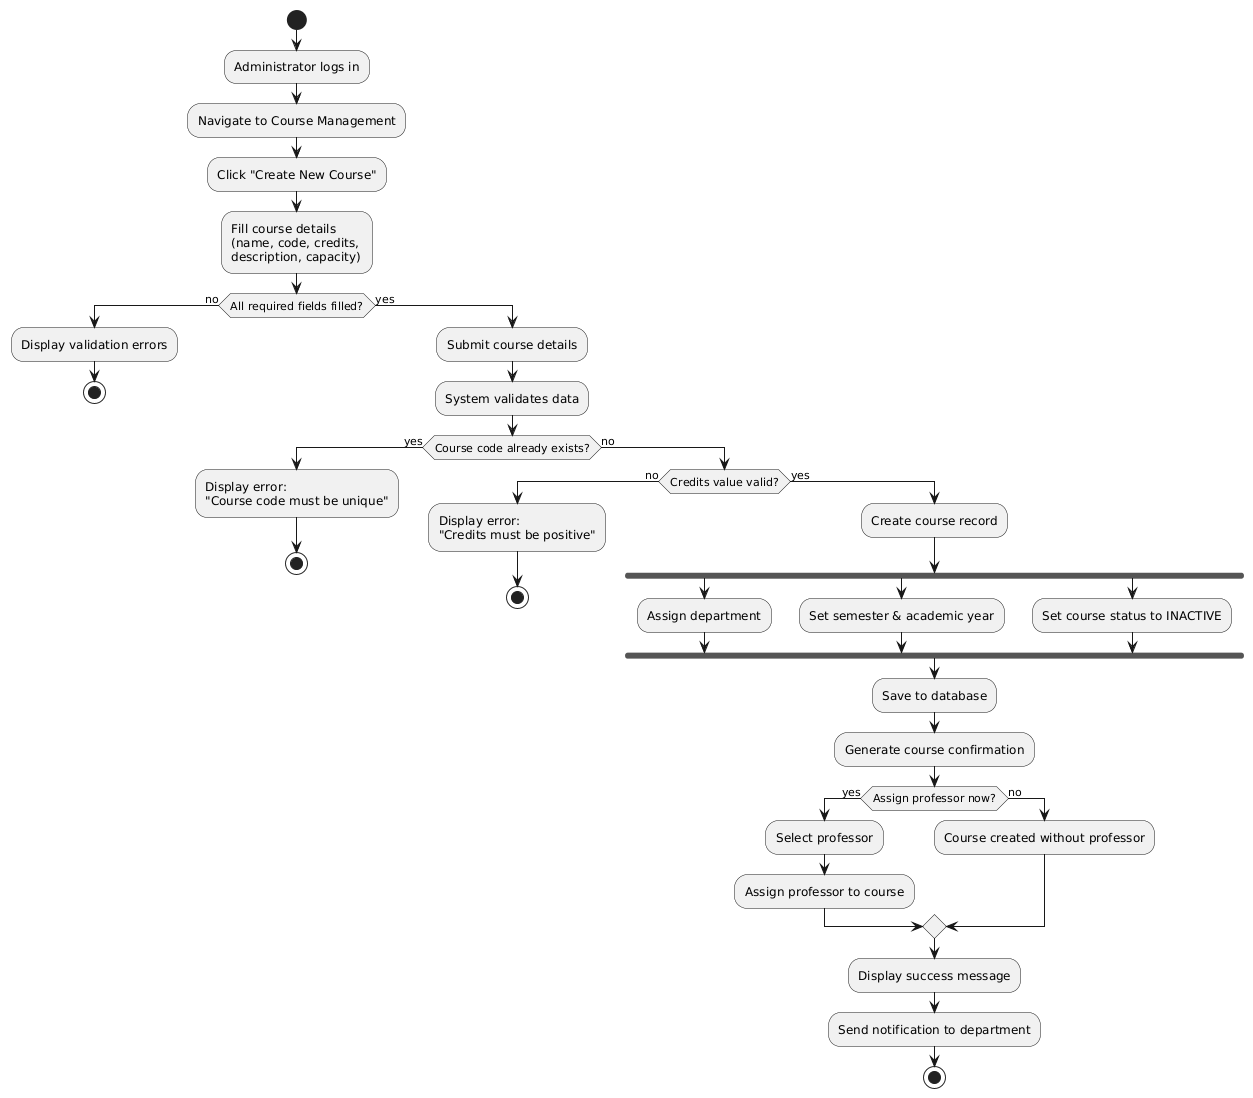
\includegraphics[width=15cm]{ACTIVITY DIAGRAM - Course Creation Process.png}
    \caption{Diagramme d'activité : Processus de création de cours}
    \label{fig:activity}
\end{figure}


% ==========================================================
% CHAPITRE 3 : SPRINT 0
% ==========================================================
\chapter{Sprint 0 : Mise en Place de l'Infrastructure}

\section{Présentation du sprint}

Le Sprint 0 correspond à la phase d'initialisation technique du projet. Il ne livre pas encore de fonctionnalité métier complète, mais il prépare les conditions nécessaires au développement incrémental : structure du dépôt, environnement de développement, socle backend, socle frontend et base de données.

Le projet analysé présente une architecture web en deux parties : un backend Spring Boot exposant des API REST sous le préfixe \texttt{/api}, et un frontend Angular organisé en modules fonctionnels chargés à la demande. L'infrastructure locale repose sur Docker Compose avec une base PostgreSQL et des configurations séparées pour l'exécution locale et l'exécution conteneurisée.

\section{Sprint Goal}

Mettre en place une infrastructure de développement reproductible permettant de lancer le backend, le frontend et la base de données, puis de démarrer les sprints fonctionnels sans blocage technique majeur.

\section{Sprint Backlog}

\begin{longtable}{|p{1.6cm}|p{6cm}|p{5.6cm}|p{1.4cm}|}
\caption{Sprint Backlog -- Sprint 0}\\
\hline
\textbf{ID} & \textbf{Élément du backlog} & \textbf{Résultat attendu} & \textbf{Pts} \\
\hline
\endfirsthead
\hline
\textbf{ID} & \textbf{Élément du backlog} & \textbf{Résultat attendu} & \textbf{Pts} \\
\hline
\endhead
S0-01 & Initialiser le dépôt et l'organisation du projet & Arborescence séparant \texttt{backend}, \texttt{frontend}, documentation et rapport & 2 \\
\hline
S0-02 & Créer le projet Spring Boot & Application Java 17 avec Web, JPA, Security, Validation, PostgreSQL et tests & 3 \\
\hline
S0-03 & Créer le projet Angular & Application Angular avec routing, modules fonctionnels et services partagés & 3 \\
\hline
S0-04 & Préparer Docker Compose & Services backend, frontend et PostgreSQL configurés pour l'exécution locale & 3 \\
\hline
S0-05 & Préparer la documentation initiale & Guides de démarrage, documentation API et notes d'intégration & 2 \\
\hline
\end{longtable}

\section{Analyse fonctionnelle}

Le Sprint 0 répond principalement à des besoins techniques. Les acteurs concernés sont les développeurs et les futurs utilisateurs indirectement, car la qualité de l'infrastructure conditionne la stabilité des modules métier.

\begin{itemize}[itemsep=0.4em]
    \item Le développeur doit pouvoir lancer le backend Spring Boot et le frontend Angular séparément ou via conteneurs.
    \item Le backend doit pouvoir accéder à une base relationnelle PostgreSQL.
    \item Le frontend doit disposer d'un proxy et d'une configuration d'environnement pour consommer les API REST.
    \item La structure du projet doit permettre l'ajout progressif des modules authentification, administrateur, professeur et étudiant.
\end{itemize}

\section{Conception du sprint}

La conception du Sprint 0 repose sur une architecture en couches. Le frontend Angular dialogue avec les contrôleurs REST du backend. Ces contrôleurs délèguent la logique aux services métier, qui utilisent les repositories JPA pour accéder aux entités persistées dans PostgreSQL.

\begin{figure}[H]
    \centering
    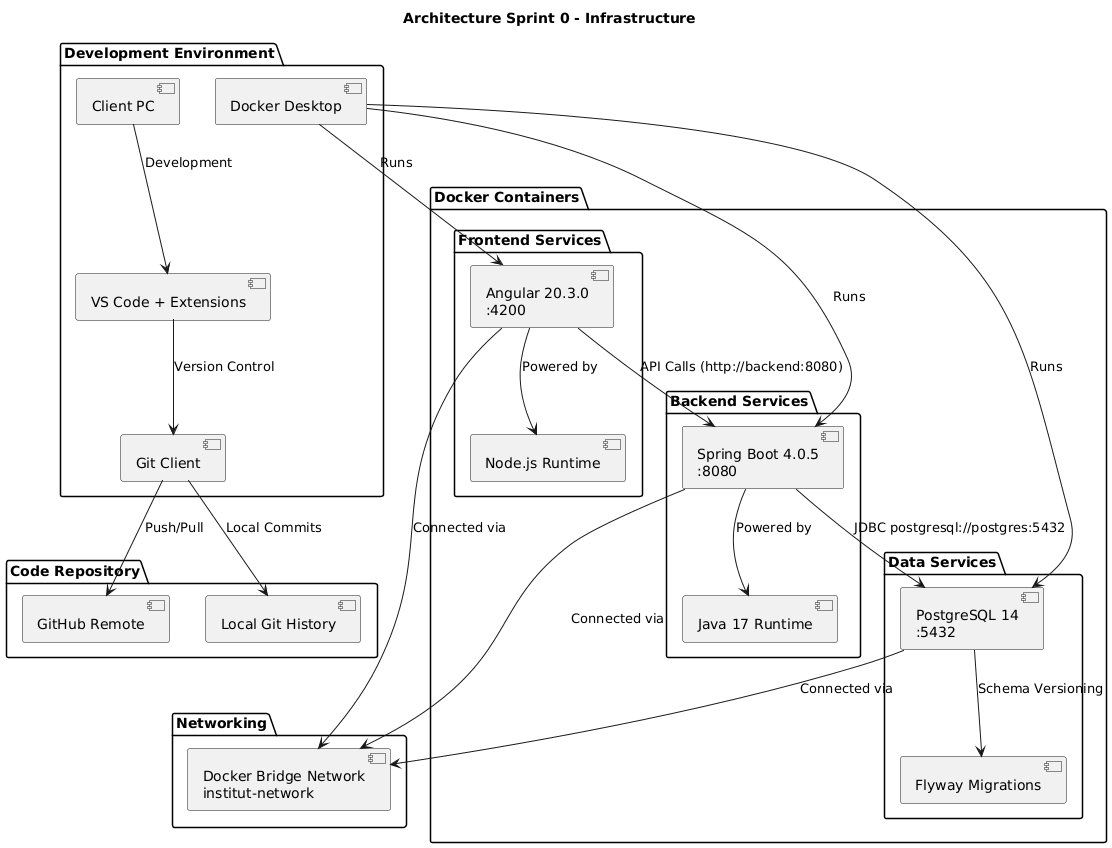
\includegraphics[width=14cm]{archDiag.png}
    \caption{Architecture technique mise en place pendant le Sprint 0}
    \label{fig:sprint0-architecture}
\end{figure}

\section{Réalisation}

Les réalisations visibles dans le dépôt sont les suivantes :

\begin{itemize}[itemsep=0.4em]
    \item création d'un backend Spring Boot dans \texttt{backend}, avec contrôleurs, services, repositories, modèles, DTO, sécurité JWT et configuration CORS ;
    \item création d'un frontend Angular dans \texttt{frontend}, avec modules \texttt{auth}, \texttt{admin}, \texttt{professor}, \texttt{student}, guards, interceptors et services partagés ;
    \item ajout d'un fichier \texttt{docker-compose.yml} pour orchestrer les services de l'application ;
    \item ajout des fichiers \texttt{application.properties}, \texttt{application-docker.properties}, \texttt{proxy.conf.js} et \texttt{proxy.conf.json} ;
    \item rédaction de documents de démarrage et d'intégration tels que \texttt{README.md}, \texttt{QUICKSTART.md}, \texttt{BACKEND\_FRONTEND\_INTEGRATION.md} et les guides backend.
\end{itemize}

\section{Tests}

La validation du Sprint 0 repose sur la capacité de compilation et de démarrage des deux applications. Le backend contient un test de contexte Spring Boot et des tests de services. Le frontend contient des tests unitaires pour les services, guards et interceptors de base.

\section{Review}

La revue du Sprint 0 a permis de valider que le socle technique était prêt pour l'authentification. L'incrément démontrable est un projet exécutable avec une séparation claire entre backend, frontend, configuration et documentation.

\section{Rétrospective}

Les points positifs du sprint sont la séparation claire des responsabilités, l'utilisation d'une architecture en couches et la présence de guides techniques. Le principal axe d'amélioration identifié est la nécessité de maintenir la documentation synchronisée avec les évolutions du code afin d'éviter les divergences entre implémentation et rapport.

\section{Bilan}

Le Sprint 0 est considéré comme terminé. Il fournit un environnement cohérent pour démarrer les développements fonctionnels et limite les risques d'intégration grâce à une structure modulaire.

\section{Sprint suivant}

Le Sprint 1 se concentre sur l'authentification complète : API de connexion, génération et validation des JWT, refresh token, stockage côté Angular, guards et redirections par rôle.

% ==========================================================
% CHAPITRE 4 : SPRINT 1
% ==========================================================
\chapter{Sprint 1 : Module authentification}

\section{Présentation du sprint}

Le Sprint 1 livre le module d'authentification côté backend et côté frontend. Il met en place la connexion par email et mot de passe, la génération de tokens JWT, le refresh token, la récupération de l'utilisateur connecté et la protection des routes Angular.

L'analyse du code montre que le backend expose les endpoints \texttt{/api/auth/login}, \texttt{/api/auth/admin/login}, \texttt{/api/auth/register}, \texttt{/api/auth/refresh}, \texttt{/api/auth/me}, \texttt{/api/auth/validate} et \texttt{/api/auth/logout}. Le frontend centralise l'état d'authentification dans \texttt{AuthService}, stocke les tokens via \texttt{StorageService}, puis sécurise les routes avec \texttt{roleGuard}.

\section{Sprint Goal}

Permettre à un administrateur, un professeur ou un étudiant de se connecter depuis l'interface Angular, recevoir un token JWT valide, conserver une session via refresh token et accéder uniquement à l'espace autorisé par son rôle.

\section{Sprint Backlog}

\begin{longtable}{|p{1.6cm}|p{6cm}|p{5.6cm}|p{1.4cm}|}
\caption{Sprint Backlog -- Sprint 1}\\
\hline
\textbf{ID} & \textbf{User Story} & \textbf{Critères d'acceptation} & \textbf{Pts} \\
\hline
\endfirsthead
\hline
\textbf{ID} & \textbf{User Story} & \textbf{Critères d'acceptation} & \textbf{Pts} \\
\hline
\endhead
S1-01 & En tant qu'utilisateur, je veux me connecter avec mon email et mon mot de passe & Le backend vérifie BCrypt, refuse les comptes inactifs et retourne un token & 8 \\
\hline
S1-02 & En tant qu'utilisateur connecté, je veux conserver ma session & Le refresh token renouvelle le token d'accès lorsque le token reste valide & 5 \\
\hline
S1-03 & En tant qu'application frontend, je veux connaître l'utilisateur connecté & L'endpoint \texttt{/me} retourne l'identifiant, l'email, le nom et le rôle & 5 \\
\hline
S1-04 & En tant qu'utilisateur, je veux être redirigé vers mon espace & Les rôles \texttt{ADMIN}, \texttt{PROFESSOR} et \texttt{STUDENT} mènent vers les routes dédiées & 6 \\
\hline
S1-05 & En tant que système, je veux protéger les routes et les API & Les routes Angular et les endpoints \texttt{/api/admin/**} appliquent les règles d'accès & 8 \\
\hline
S1-06 & En tant que développeur, je veux tester les services d'authentification & Les tests couvrent services, guards et interceptors côté frontend & 3 \\
\hline
\end{longtable}

\section{Analyse fonctionnelle}

Les acteurs du sprint sont l'utilisateur non connecté, l'administrateur, le professeur et l'étudiant. Le besoin central est la création d'une session sécurisée et contextualisée par rôle.

\begin{itemize}[itemsep=0.4em]
    \item L'utilisateur saisit ses identifiants dans la page d'authentification Angular.
    \item Le backend vérifie l'existence du compte, le mot de passe haché et l'état actif du compte.
    \item Le système génère un JWT contenant l'email, l'identifiant et le type d'utilisateur.
    \item Le frontend stocke les tokens, expose l'état de session et ajoute automatiquement le header \texttt{Authorization}.
    \item Les guards empêchent l'accès aux espaces non autorisés.
\end{itemize}

\section{Conception du sprint}

\subsection*{Diagramme de cas d'utilisation}

\begin{figure}[H]
\centering
\begin{tikzpicture}[node distance=1.2cm and 1.6cm, scale=0.82, transform shape]
    \node[sprintactor] (visitor) {Utilisateur};
    \node[sprintcase, right=3.0cm of visitor] (login) {Se connecter};
    \node[sprintcase, above=of login] (validate) {Valider les\\identifiants};
    \node[sprintcase, below=of login] (refresh) {Renouveler\\la session};
    \node[sprintcase, right=2.4cm of login] (access) {Accéder à\\un espace protégé};
    \node[sprintactor, right=2.5cm of access] (system) {Système\\JWT/RBAC};
    \node[sprintboundary, fit=(validate)(login)(refresh)(access), label=above:{Module authentification}] {};

    \draw[sprintline] (visitor) -- (login);
    \draw[sprintarrow] (login) -- (validate);
    \draw[sprintarrow] (login) -- (refresh);
    \draw[sprintarrow] (login) -- (access);
    \draw[sprintline] (system) -- (access);
\end{tikzpicture}
\caption{Cas d'utilisation du module authentification}
\label{fig:sprint1-usecase}
\end{figure}

\subsection*{Diagramme de séquence}

\begin{figure}[H]
    \centering
    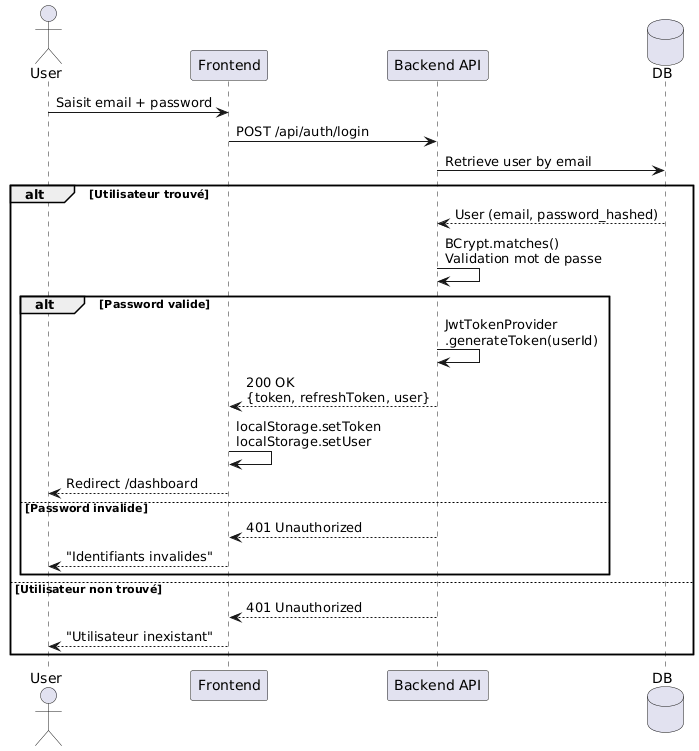
\includegraphics[width=14cm]{FluxLogin(sequence).png}
    \caption{Flux de connexion utilisateur}
    \label{fig:sprint1-login-sequence}
\end{figure}

\subsection*{Diagramme de classes}

\begin{figure}[H]
    \centering
    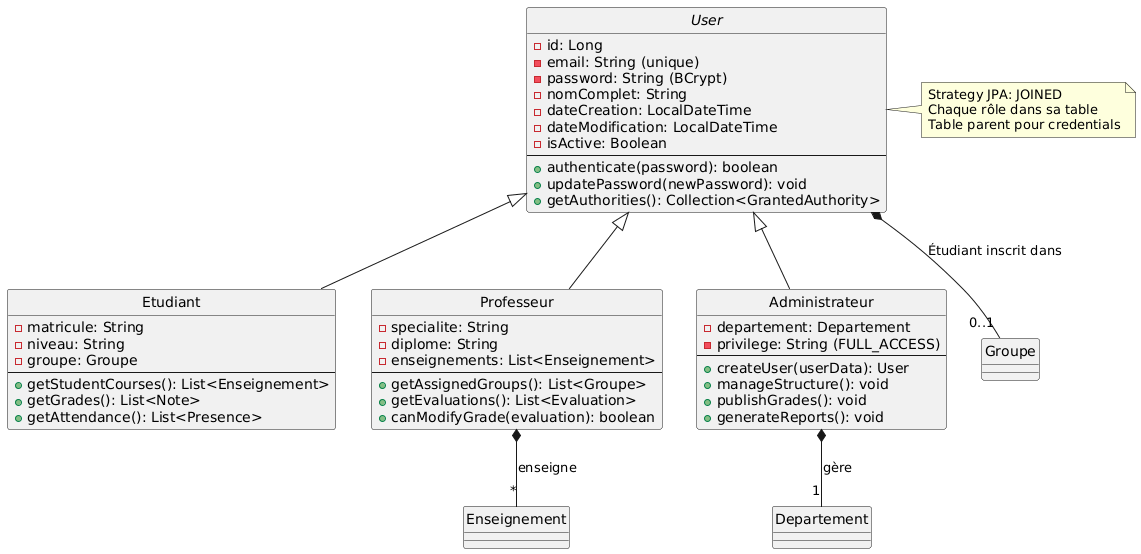
\includegraphics[width=13cm]{userdataDiag.png}
    \caption{Modèle utilisateur et spécialisation par rôle}
    \label{fig:sprint1-user-classes}
\end{figure}

\subsection*{Diagramme d'état}

\begin{figure}[H]
    \centering
    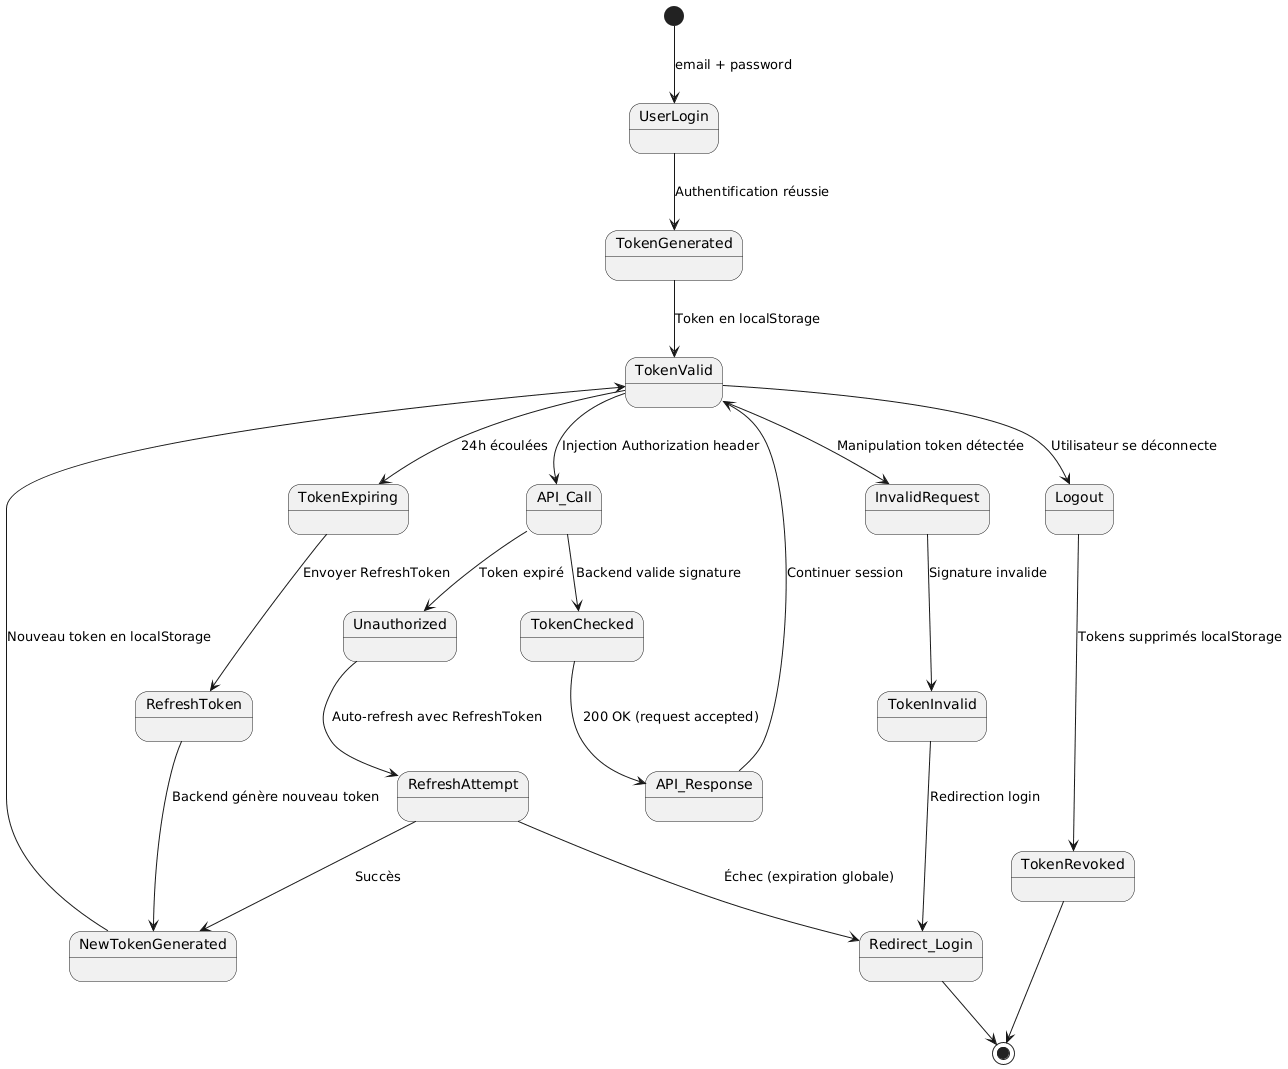
\includegraphics[width=13cm]{Diagdetat.png}
    \caption{Cycle de vie du token JWT}
    \label{fig:sprint1-token-state}
\end{figure}

\section{Réalisation}

Côté backend, la réalisation s'appuie sur \texttt{AuthController}, \texttt{AuthService}, \texttt{JwtTokenProvider}, \texttt{JwtAuthenticationFilter} et \texttt{SecurityConfig}. Les mots de passe sont vérifiés avec BCrypt. Les comptes héritent de l'entité \texttt{User} selon la stratégie JPA \texttt{JOINED}, avec les spécialisations \texttt{Administrateur}, \texttt{Professeur} et \texttt{Etudiant}.

Côté frontend, la page \texttt{AuthPageComponent} utilise un formulaire réactif et des signaux Angular pour gérer l'état de soumission. \texttt{AuthApiService} consomme les endpoints REST, \texttt{AuthService} maintient l'état de session, \texttt{JwtInterceptor} ajoute le token aux requêtes et \texttt{ErrorInterceptor} gère les erreurs HTTP.

\section{Tests}

Les tests existants couvrent les services Angular d'authentification, le stockage local, les guards et les interceptors. Côté backend, la validation repose sur les tests Spring Boot et sur les guides d'exécution des flux JWT présents dans le dossier backend.

\section{Review}

La revue valide que le module authentification est utilisable de bout en bout : formulaire de connexion, token, refresh token, récupération de l'utilisateur connecté et redirection selon le rôle.

\section{Rétrospective}

Le sprint a confirmé l'intérêt de centraliser l'état d'authentification dans un service Angular unique. L'amélioration prioritaire pour les sprints suivants est de réutiliser systématiquement les guards et les interceptors afin d'éviter une logique de sécurité dispersée.

\section{Bilan}

Le Sprint 1 fournit le socle de sécurité nécessaire aux modules métier. Les espaces administrateur, professeur et étudiant peuvent désormais être protégés par rôle et consommer les API avec un token JWT.

\section{Sprint suivant}

Le Sprint 2 exploite ce socle pour livrer le module administrateur, avec dashboard, structure académique, planification des examens, validation des notes et supervision des présences.

% ==========================================================
% CHAPITRE 5 : SPRINT 2
% ==========================================================
\chapter{Sprint 2 : Module administrateur}

\section{Présentation du sprint}

Le Sprint 2 est consacré au module administrateur, côté backend et côté frontend. L'objectif est de fournir à l'administration une vue de pilotage et des actions de gestion sur les données académiques principales.

Dans le code, ce module repose sur les endpoints \texttt{/api/admin/dashboard}, \texttt{/api/admin/academic-years}, \texttt{/api/admin/exam-planning}, \texttt{/api/admin/note-validation} et \texttt{/api/admin/attendance-supervision}. Le frontend correspondant est \texttt{AdminDashboardComponent}, alimenté par \texttt{AdminDashboardApi}.

\section{Sprint Goal}

Livrer un espace administrateur sécurisé permettant de consulter les indicateurs globaux, gérer les années et semestres académiques, planifier et publier les examens, valider ou rejeter les notes soumises et superviser les présences.

\section{Sprint Backlog}

\begin{longtable}{|p{1.6cm}|p{6cm}|p{5.6cm}|p{1.4cm}|}
\caption{Sprint Backlog -- Sprint 2}\\
\hline
\textbf{ID} & \textbf{User Story} & \textbf{Critères d'acceptation} & \textbf{Pts} \\
\hline
\endfirsthead
\hline
\textbf{ID} & \textbf{User Story} & \textbf{Critères d'acceptation} & \textbf{Pts} \\
\hline
\endhead
S2-01 & En tant qu'administrateur, je veux consulter un tableau de bord global & Les statistiques étudiants, professeurs, cours et groupes sont affichées & 5 \\
\hline
S2-02 & En tant qu'administrateur, je veux gérer les années et semestres & Création, activation, verrouillage et consultation sont disponibles & 7 \\
\hline
S2-03 & En tant qu'administrateur, je veux planifier des examens & Les examens peuvent être créés, créés en masse et publiés & 7 \\
\hline
S2-04 & En tant qu'administrateur, je veux valider les notes & Les notes soumises peuvent être validées, rejetées ou publiées & 8 \\
\hline
S2-05 & En tant qu'administrateur, je veux superviser les présences & Les séances peuvent être clôturées, rouvertes et les éliminations suivies & 6 \\
\hline
S2-06 & En tant qu'administrateur, je veux filtrer les données dans l'interface & Les filtres par département, groupe, rôle et recherche sont disponibles & 2 \\
\hline
\end{longtable}

\section{Analyse fonctionnelle}

Le module administrateur couvre les besoins de pilotage académique et de contrôle. Il ne remplace pas tous les CRUD génériques du backend, mais il assemble les informations utiles à la prise de décision et aux validations pédagogiques.

\begin{itemize}[itemsep=0.4em]
    \item Consultation des indicateurs agrégés via \texttt{AdminDashboardService}.
    \item Gestion du calendrier académique via \texttt{AcademicYearController}.
    \item Planification et publication des examens via \texttt{ExamPlanningController}.
    \item Validation du workflow de notes via \texttt{NoteValidationController} et \texttt{NoteWorkflowService}.
    \item Supervision des présences, absences collectives et éliminations via \texttt{AttendanceSupervisionController}.
\end{itemize}

\section{Conception du sprint}

\subsection*{Diagramme de cas d'utilisation}

\begin{figure}[H]
\centering
\begin{tikzpicture}[node distance=1.05cm and 1.45cm, scale=0.84, transform shape]
    \node[sprintactor] (admin) {Administrateur};
    \node[sprintcase, right=3.0cm of admin] (dash) {Consulter\\dashboard};
    \node[sprintcase, above=of dash] (year) {Gérer années\\et semestres};
    \node[sprintcase, right=2.3cm of dash] (exam) {Planifier et\\publier examens};
    \node[sprintcase, below=of dash] (notes) {Valider et\\publier notes};
    \node[sprintcase, below=of exam] (att) {Superviser\\présences};
    \node[sprintboundary, fit=(year)(dash)(notes)(exam)(att), label=above:{Espace administrateur}] {};

    \draw[sprintline] (admin) -- (dash);
    \draw[sprintline] (admin) |- (year);
    \draw[sprintline] (admin) |- (notes);
    \draw[sprintline] (admin) -- (exam);
    \draw[sprintline] (admin) |- (att);
\end{tikzpicture}
\caption{Cas d'utilisation du module administrateur}
\label{fig:sprint2-usecase}
\end{figure}

\subsection*{Diagramme de classes simplifié}

\begin{figure}[H]
\centering
\begin{tikzpicture}[node distance=1.0cm and 1.1cm]
    \node[sprintclass] (ay) {\textbf{AcademicYear}\\id, label, startDate\\endDate, active};
    \node[sprintclass, right=of ay] (sem) {\textbf{Semester}\\id, name, startDate\\endDate, active, locked};
    \node[sprintclass, below=of ay] (eva) {\textbf{Evaluation}\\id, libelle, type\\dateEvaluation\\planningStatus};
    \node[sprintclass, right=of eva] (note) {\textbf{Note}\\id, valeur, statut\\submittedAt\\validatedAt\\publishedAt};
    \node[sprintclass, below=of eva] (seance) {\textbf{Seance}\\id, jour, heures\\typeSeance\\attendanceStatus};
    \node[sprintclass, right=of seance] (elim) {\textbf{EliminationRecord}\\id, absenceCount\\status, detectedAt\\notifiedAt};
    \draw[sprintline] (ay) -- node[above, font=\scriptsize]{1} node[below, font=\scriptsize]{contient} node[above right, font=\scriptsize]{0..n} (sem);
    \draw[sprintline] (eva) -- node[above, font=\scriptsize]{1} node[below, font=\scriptsize]{possède} node[above right, font=\scriptsize]{0..n} (note);
    \draw[sprintline] (seance) -- node[left, font=\scriptsize]{planifie} (eva);
    \draw[sprintline] (seance) -- node[above, font=\scriptsize]{déclenche} (elim);
\end{tikzpicture}
\caption{Classes principales mobilisées par le module administrateur}
\label{fig:sprint2-classes}
\end{figure}

\subsection*{Diagramme de séquence -- validation des notes}

\begin{figure}[H]
\centering
\begin{tikzpicture}[node distance=1.0cm and 1.0cm, scale=0.82, transform shape]
    \node[sprintseq] (ui) {AdminDashboard};
    \node[sprintseq, right=of ui] (api) {AdminDashboardApi};
    \node[sprintseq, right=of api] (ctrl) {NoteValidationController};
    \node[sprintseq, right=of ctrl] (svc) {NoteValidationService};
    \node[sprintseq, right=of svc] (repo) {Repositories};

    \foreach \x in {ui,api,ctrl,svc,repo}
        \draw[dashed, gray] (\x.south) -- ++(0,-3.0);

    \draw[sprintarrow] ([yshift=-0.7cm]ui.south) -- node[above, font=\scriptsize]{choisir décision} ([yshift=-0.7cm]api.south);
    \draw[sprintarrow] ([yshift=-1.3cm]api.south) -- node[above, font=\scriptsize]{PATCH validation/rejet/publication} ([yshift=-1.3cm]ctrl.south);
    \draw[sprintarrow] ([yshift=-1.9cm]ctrl.south) -- node[above, font=\scriptsize]{appliquer workflow} ([yshift=-1.9cm]svc.south);
    \draw[sprintarrow] ([yshift=-2.5cm]svc.south) -- node[above, font=\scriptsize]{sauvegarder notes} ([yshift=-2.5cm]repo.south);
\end{tikzpicture}
\caption{Séquence de validation ou publication des notes}
\label{fig:sprint2-note-validation-sequence}
\end{figure}

\section{Réalisation}

Côté backend, les services \texttt{AdminDashboardService}, \texttt{AcademicYearService}, \texttt{ExamPlanningService}, \texttt{NoteValidationService}, \texttt{AttendanceSupervisionService} et \texttt{AttendanceEliminationService} concentrent la logique métier du module. Les DTO spécialisés évitent d'exposer directement les entités JPA dans les tableaux de bord.

Côté frontend, \texttt{AdminDashboardComponent} utilise les signaux Angular pour gérer les sections actives, les chargements, les filtres, la planification d'examens, la validation des notes et la supervision des présences. Le service \texttt{AdminDashboardApi} regroupe les appels HTTP vers les endpoints administrateur.

\section{Tests}

Les tests automatisés existants couvrent notamment le contexte Spring Boot, certains services backend et les services/guards/interceptors Angular. La validation fonctionnelle du Sprint 2 consiste à vérifier la protection de la route \texttt{/admin}, la récupération du dashboard, la création/activation d'une année académique, la planification d'examens, la validation de notes et la supervision des absences.

\section{Review}

La revue du Sprint 2 confirme que l'administrateur dispose d'un espace centralisé connecté au backend. Les workflows critiques de validation des notes et de supervision des présences sont présents dans le code et accessibles via des endpoints dédiés.

\section{Rétrospective}

Le découpage par endpoints administrateur a facilité l'intégration frontend. Le principal point d'amélioration est de renforcer les tests automatisés sur les workflows administratifs complexes, notamment la publication d'examens et la validation de notes.

\section{Bilan}

Le Sprint 2 transforme le socle authentifié en outil de pilotage administratif. Les principales entités académiques sont consultées ou contrôlées depuis l'espace administrateur, avec une logique métier centralisée côté backend.

\section{Sprint suivant}

Le Sprint 3 se concentre sur le module professeur : consultation des enseignements, gestion des séances, saisie des notes, enregistrement des présences, création de rattrapages et dépôt des supports.

% ==========================================================
% CHAPITRE 6 : SPRINT 3
% ==========================================================
\chapter{Sprint 3 : Module professeur}

\section{Présentation du sprint}

Le Sprint 3 livre le module professeur côté backend et côté frontend. Il donne au professeur une interface de suivi de ses enseignements, groupes, séances, évaluations, notes, présences et supports de cours.

Le backend expose notamment \texttt{/api/professor/dashboard}, \texttt{/api/professor/evaluations} et \texttt{/api/professor/attendance/\{sessionId\}/collective-absence}. Le module utilise aussi les endpoints transverses \texttt{/api/notes}, \texttt{/api/presences}, \texttt{/api/schedules} et \texttt{/api/supports/upload}. Le frontend correspondant est \texttt{ProfessorDashboardComponent}, alimenté par \texttt{ProfessorDashboardApi}.

\section{Sprint Goal}

Permettre au professeur connecté de consulter ses données pédagogiques, créer et gérer ses évaluations, saisir ou soumettre les notes, enregistrer les présences de manière optimisée, signaler une absence collective, créer des séances de rattrapage et déposer des supports de cours.

\section{Sprint Backlog}

\begin{longtable}{|p{1.6cm}|p{6cm}|p{5.6cm}|p{1.4cm}|}
\caption{Sprint Backlog -- Sprint 3}\\
\hline
\textbf{ID} & \textbf{User Story} & \textbf{Critères d'acceptation} & \textbf{Pts} \\
\hline
\endfirsthead
\hline
\textbf{ID} & \textbf{User Story} & \textbf{Critères d'acceptation} & \textbf{Pts} \\
\hline
\endhead
S3-01 & En tant que professeur, je veux consulter mon dashboard & Enseignements, groupes, séances, évaluations et supports sont chargés & 6 \\
\hline
S3-02 & En tant que professeur, je veux saisir des notes & Les notes sont créées ou soumises via l'API \texttt{/api/notes} & 8 \\
\hline
S3-03 & En tant que professeur, je veux enregistrer les présences rapidement & Tous les étudiants sont présents par défaut et seuls les absents sont marqués avant sauvegarde via \texttt{/api/presences} & 7 \\
\hline
S3-04 & En tant que professeur, je veux signaler une absence collective & Le statut de la séance passe à \texttt{SIGNALEE} si la séance appartient au professeur & 5 \\
\hline
S3-05 & En tant que professeur, je veux créer un rattrapage & Une séance de type rattrapage est créée via \texttt{/api/schedules} & 4 \\
\hline
S3-06 & En tant que professeur, je veux déposer des supports & L'upload multipart enregistre fichier, métadonnées et enseignement associé & 5 \\
\hline
S3-07 & En tant que professeur, je veux créer et gérer mes évaluations & Les évaluations peuvent être créées, modifiées ou supprimées via les endpoints professeur avec contrôle d'appartenance & 5 \\
\hline
\end{longtable}

\section{Analyse fonctionnelle}

Le professeur agit sur les données liées à ses enseignements. Le système récupère le professeur à partir de l'email présent dans le token JWT, puis construit une réponse de synthèse à partir des enseignements, séances, évaluations, étudiants, notes, présences et supports.

\begin{itemize}[itemsep=0.4em]
    \item Consultation des modules et groupes affectés.
    \item Consultation des séances et évaluations académiques.
    \item Création, modification et suppression des évaluations liées aux enseignements du professeur.
    \item Saisie de notes avec statut de brouillon ou de soumission.
    \item Saisie optimisée des présences : tous les étudiants sont présents par défaut et le professeur marque uniquement les absents.
    \item Dépôt de supports de cours avec stockage de fichier.
\end{itemize}

\section{Conception du sprint}

\subsection*{Diagramme de cas d'utilisation}

\begin{figure}[H]
\centering
\begin{tikzpicture}[node distance=1.05cm and 1.45cm, scale=0.84, transform shape]
    \node[sprintactor] (prof) {Professeur};
    \node[sprintcase, right=3.0cm of prof] (dash) {Consulter\\dashboard};
    \node[sprintcase, above=of dash] (grades) {Saisir et\\soumettre notes};
    \node[sprintcase, right=2.4cm of dash] (attendance) {Gérer\\présences};
    \node[sprintcase, above=of attendance] (evals) {Gérer\\évaluations};
    \node[sprintcase, below=of dash] (makeup) {Créer\\rattrapage};
    \node[sprintcase, below=of attendance] (upload) {Déposer\\support};
    \node[sprintboundary, fit=(evals)(grades)(dash)(makeup)(attendance)(upload), label=above:{Espace professeur}] {};

    \draw[sprintline] (prof) -- (dash);
    \draw[sprintline] (prof) |- (grades);
    \draw[sprintline] (prof) |- (evals);
    \draw[sprintline] (prof) -- (attendance);
    \draw[sprintline] (prof) |- (makeup);
    \draw[sprintline] (prof) |- (upload);
\end{tikzpicture}
\caption{Cas d'utilisation du module professeur}
\label{fig:sprint3-usecase}
\end{figure}

\subsection*{Diagramme de séquence -- saisie de notes}

\begin{figure}[H]
    \centering
    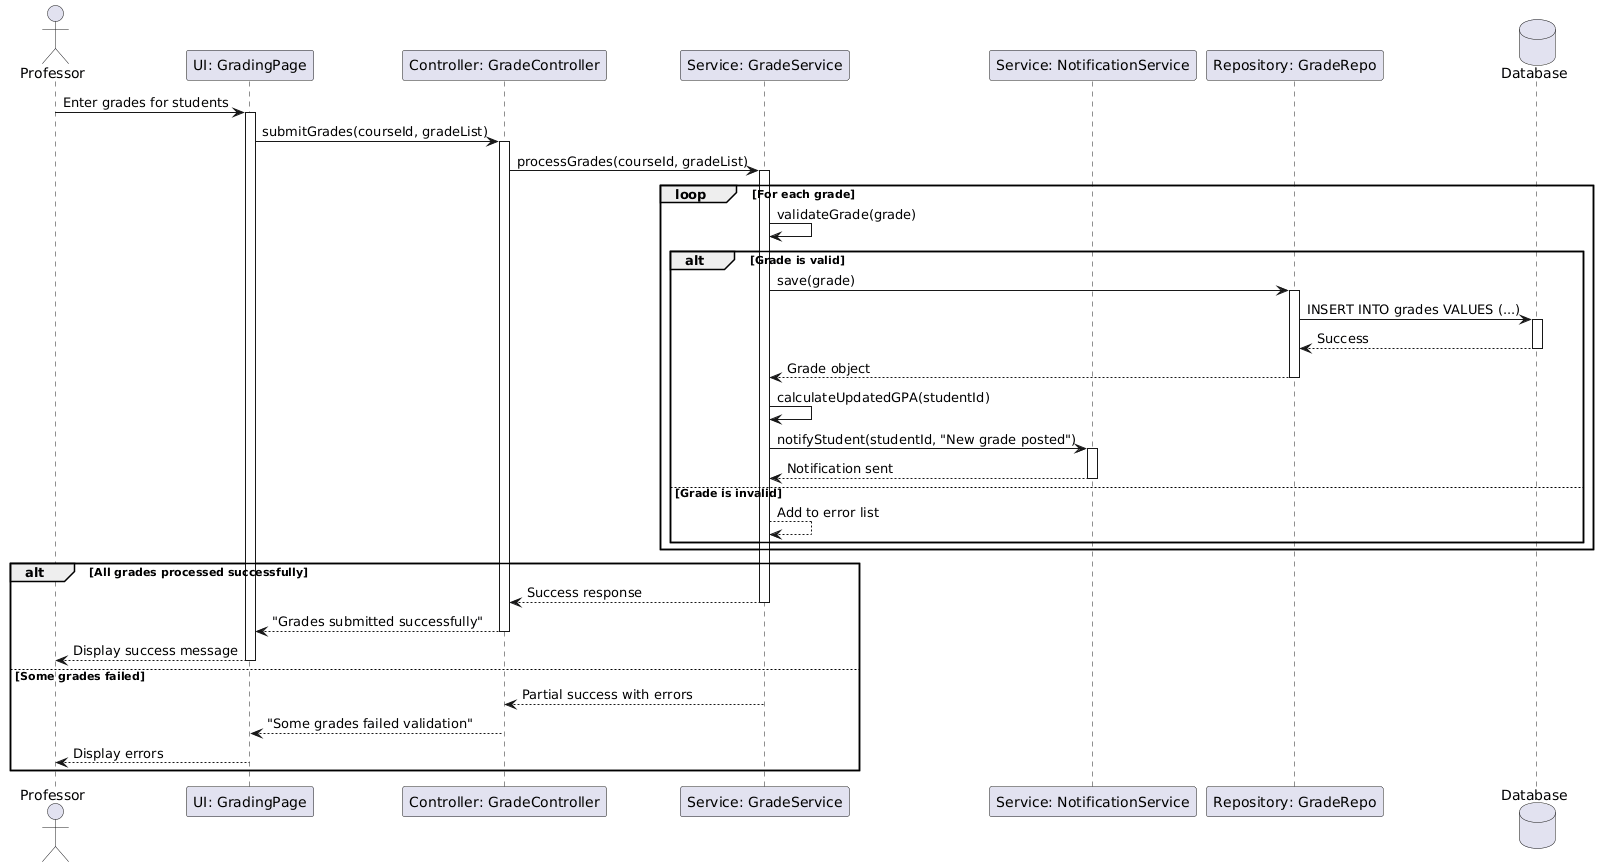
\includegraphics[width=14cm]{SEQUENCE DIAGRAM - Professor Grade Entry.png}
    \caption{Séquence de saisie des notes par le professeur}
    \label{fig:sprint3-grade-sequence}
\end{figure}

\subsection*{Diagramme d'activité -- dépôt d'un support}

\begin{figure}[H]
\centering
\begin{tikzpicture}[node distance=0.75cm]
    \node[sprintstart] (start) {};
    \node[sprintactivity, below=of start] (teaching) {Choisir un enseignement};
    \node[sprintactivity, below=of teaching] (file) {Sélectionner un fichier};
    \node[sprintdecision, below=of file] (valid) {Fichier\\valide ?};
    \node[sprintactivity, below=of valid] (send) {Envoyer la requête multipart};
    \node[sprintactivity, below=of send] (store) {Stocker le fichier et les métadonnées};
    \node[sprintactivity, below=of store] (refresh) {Rafraîchir les supports affichés};
    \node[sprintend, below=of refresh] (end) {};
    \node[sprintactivity, right=2.4cm of valid] (error) {Afficher un message d'erreur};

    \draw[sprintarrow] (start) -- (teaching);
    \draw[sprintarrow] (teaching) -- (file);
    \draw[sprintarrow] (file) -- (valid);
    \draw[sprintarrow] (valid) -- node[right, font=\scriptsize]{Oui} (send);
    \draw[sprintarrow] (send) -- (store);
    \draw[sprintarrow] (store) -- (refresh);
    \draw[sprintarrow] (refresh) -- (end);
    \draw[sprintarrow] (valid) -- node[above, font=\scriptsize]{Non} (error);
\end{tikzpicture}
\caption{Activité de dépôt d'un support de cours}
\label{fig:sprint3-upload-activity}
\end{figure}

\section{Réalisation}

Côté backend, \texttt{ProfessorDashboardService} agrège les données du professeur connecté. Il construit les statistiques, enseignements, groupes, séances, évaluations, étudiants, notes, présences et supports. Il contrôle aussi la création, la modification et la suppression des évaluations via les endpoints professeur, avec vérification que l'enseignement appartient bien au professeur connecté. La saisie de notes s'appuie sur \texttt{NoteService} et \texttt{NoteWorkflowService}. Les présences utilisent \texttt{PresenceService}. Le dépôt de fichiers repose sur \texttt{SupportCoursService} et \texttt{FileStorageService}.

Côté frontend, \texttt{ProfessorDashboardComponent} gère l'état des sections avec des signaux Angular : aperçu, enseignements, groupes, emploi du temps, évaluations, notes, présences et supports. La section présence a été simplifiée : les étudiants sont considérés présents par défaut, et le professeur marque seulement les absents avant l'envoi vers l'API.

\section{Tests}

La validation du Sprint 3 couvre la route \texttt{/professor}, le chargement du dashboard, la création et la gestion des évaluations, la saisie de notes, l'enregistrement optimisé des présences avec les statuts \texttt{PRESENT} et \texttt{ABSENT}, le signalement d'une absence collective, la création de rattrapage et l'upload de supports. Le dépôt contient aussi des tests ciblés sur le stockage de fichiers et la logique de séances.

\section{Review}

La revue montre que le professeur peut suivre ses groupes et réaliser les actions pédagogiques principales depuis une interface unique. La gestion des évaluations et l'appel de présence optimisé réduisent le temps de saisie tout en conservant une trace claire des données envoyées au backend.

\section{Rétrospective}

La centralisation du dashboard professeur a simplifié le frontend. Le point à améliorer est la granularité des tests d'intégration pour vérifier les autorisations fines, par exemple empêcher un professeur d'agir sur une séance qui ne lui appartient pas.

\section{Bilan}

Le Sprint 3 livre un espace professeur exploitable. Les workflows d'évaluations, de notes, de présences optimisées, de rattrapages et de supports sont présents et connectés aux services backend.

\section{Sprint suivant}

Le Sprint 4 se concentre sur le module étudiant, principalement orienté consultation : profil, notes publiées, emploi du temps, supports, annonces, rattrapages et absences.

% ==========================================================
% CHAPITRE 7 : SPRINT 4
% ==========================================================
\chapter{Sprint 4 : Module étudiant}

\section{Présentation du sprint}

Le Sprint 4 livre le module étudiant côté backend et côté frontend. Il permet à l'étudiant connecté de consulter les informations disponibles pour son groupe, avec les annonces affichées par défaut dès l'entrée dans l'espace étudiant.

Le backend expose \texttt{/api/student/dashboard}. Le service \texttt{StudentDashboardService} construit la réponse à partir du profil étudiant, de son groupe, des séances visibles, des notes publiées, des supports, des annonces, des rattrapages, des examens publiés et des absences. Le frontend correspondant est \texttt{StudentDashboardComponent}, alimenté par \texttt{StudentDashboardApi}.

\section{Sprint Goal}

Permettre à l'étudiant de consulter depuis un espace protégé les annonces publiées par défaut, les notifications importantes, son profil, ses notes publiées, son emploi du temps, le calendrier des examens publiés, les supports de cours, les rattrapages et son suivi de présence.

\section{Sprint Backlog}

\begin{longtable}{|p{1.6cm}|p{6cm}|p{5.6cm}|p{1.4cm}|}
\caption{Sprint Backlog -- Sprint 4}\\
\hline
\textbf{ID} & \textbf{User Story} & \textbf{Critères d'acceptation} & \textbf{Pts} \\
\hline
\endfirsthead
\hline
\textbf{ID} & \textbf{User Story} & \textbf{Critères d'acceptation} & \textbf{Pts} \\
\hline
\endhead
S4-01 & En tant qu'étudiant, je veux consulter mon profil & Nom, email, matricule, niveau, groupe, département et année sont affichés & 4 \\
\hline
S4-02 & En tant qu'étudiant, je veux consulter mes notes publiées & Seules les notes avec statut publié sont visibles & 6 \\
\hline
S4-03 & En tant qu'étudiant, je veux consulter mon emploi du temps & Les séances ordinaires du groupe sont affichées hors examens & 5 \\
\hline
S4-04 & En tant qu'étudiant, je veux télécharger les supports & Les supports liés aux enseignements du groupe sont listés avec une URL de téléchargement & 4 \\
\hline
S4-05 & En tant qu'étudiant, je veux consulter les annonces & Seules les annonces publiées et visibles pour le rôle étudiant sont affichées & 3 \\
\hline
S4-06 & En tant qu'étudiant, je veux suivre mes absences & Le taux de présence et les résumés d'absence par matière sont consultables & 3 \\
\hline
S4-07 & En tant qu'étudiant, je veux être notifié des informations importantes & Un badge regroupe annonces, notes publiées, rattrapages et examens & 4 \\
\hline
S4-08 & En tant qu'étudiant, je veux consulter le calendrier des examens & Les examens publiés sont affichés dans une section dédiée & 4 \\
\hline
S4-09 & En tant qu'étudiant, je veux consulter les rattrapages & Les séances de rattrapage sont affichées dans une section dédiée & 3 \\
\hline
\end{longtable}

\section{Analyse fonctionnelle}

Le module étudiant est essentiellement consultatif. Il applique les règles de publication déjà définies dans les sprints précédents : les notes non publiées ne sont pas visibles, les examens ne sont affichés que lorsque leur planification est publiée, et les annonces sont filtrées par rôle et validité temporelle. L'interface privilégie les informations urgentes : les annonces sont affichées par défaut, une icône de notification synthétise les nouveautés importantes, et les rattrapages ainsi que les examens disposent de sections séparées.

\section{Conception du sprint}

\subsection*{Diagramme de cas d'utilisation}

\begin{figure}[H]
\centering
\begin{tikzpicture}[node distance=1.05cm and 1.45cm, scale=0.84, transform shape]
    \node[sprintactor] (student) {Étudiant};
    \node[sprintcase, right=3.0cm of student] (profile) {Consulter\\profil};
    \node[sprintcase, above=of profile] (grades) {Consulter\\notes publiées};
    \node[sprintcase, right=2.4cm of profile] (schedule) {Consulter\\emploi du temps};
    \node[sprintcase, above=of schedule] (announcements) {Consulter\\annonces};
    \node[sprintcase, below=of profile] (materials) {Télécharger\\supports};
    \node[sprintcase, below=of schedule] (attendance) {Suivre\\absences};
    \node[sprintcase, below=of materials] (makeups) {Consulter\\rattrapages};
    \node[sprintcase, right=2.4cm of grades] (exams) {Consulter\\examens};
    \node[sprintboundary, fit=(announcements)(exams)(grades)(profile)(materials)(makeups)(schedule)(attendance), label=above:{Espace étudiant}] {};

    \draw[sprintline] (student) -- (profile);
    \draw[sprintline] (student) |- (grades);
    \draw[sprintline] (student) |- (announcements);
    \draw[sprintline] (student) |- (exams);
    \draw[sprintline] (student) -- (schedule);
    \draw[sprintline] (student) |- (materials);
    \draw[sprintline] (student) |- (attendance);
    \draw[sprintline] (student) |- (makeups);
\end{tikzpicture}
\caption{Cas d'utilisation du module étudiant}
\label{fig:sprint4-usecase}
\end{figure}

\subsection*{Diagramme de séquence -- consultation des notes}

\begin{figure}[H]
    \centering
    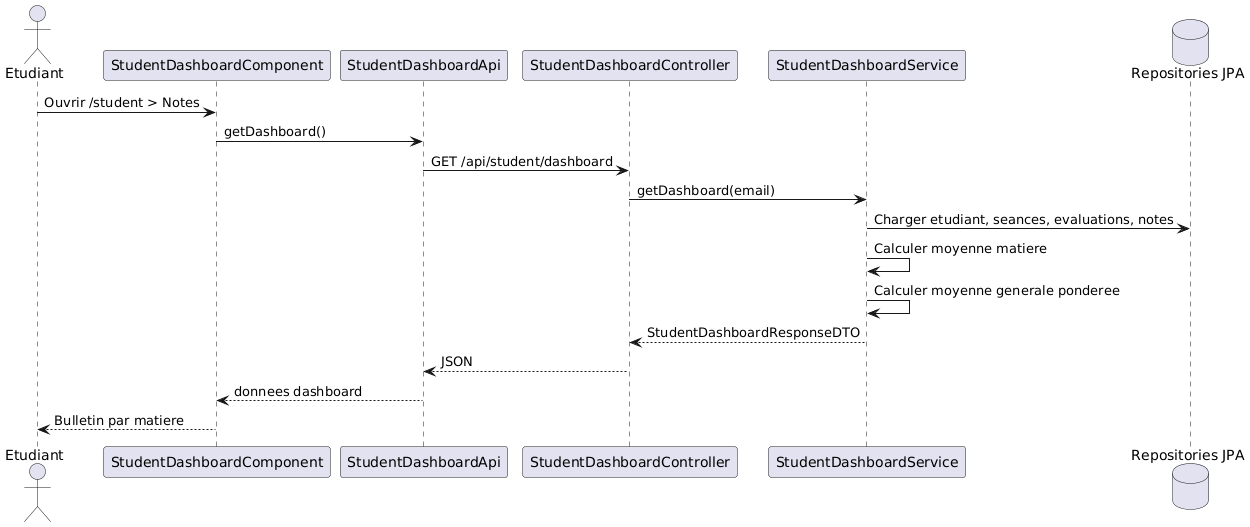
\includegraphics[width=14cm]{Diagrammesequence-consultationnotes.png}
    \caption{Séquence de consultation des notes publiées}
    \label{fig:sprint4-grade-sequence}
\end{figure}

\subsection*{Diagramme d'activité -- chargement de l'espace étudiant}

\begin{figure}[H]
\centering
\begin{tikzpicture}[node distance=0.75cm]
    \node[sprintstart] (start) {};
    \node[sprintactivity, below=of start] (auth) {Vérifier la session};
    \node[sprintdecision, below=of auth] (logged) {Session\\valide ?};
    \node[sprintactivity, below=of logged] (load) {Appeler \texttt{/api/student/dashboard}};
    \node[sprintactivity, below=of load] (filter) {Filtrer notes, examens et annonces};
    \node[sprintactivity, below=of filter] (avg) {Calculer moyennes et notifications};
    \node[sprintactivity, below=of avg] (display) {Afficher annonces par défaut et sections dédiées};
    \node[sprintend, below=of display] (end) {};
    \node[sprintactivity, right=2.4cm of logged] (redirect) {Rediriger vers la connexion};

    \draw[sprintarrow] (start) -- (auth);
    \draw[sprintarrow] (auth) -- (logged);
    \draw[sprintarrow] (logged) -- node[right, font=\scriptsize]{Oui} (load);
    \draw[sprintarrow] (load) -- (filter);
    \draw[sprintarrow] (filter) -- (avg);
    \draw[sprintarrow] (avg) -- (display);
    \draw[sprintarrow] (display) -- (end);
    \draw[sprintarrow] (logged) -- node[above, font=\scriptsize]{Non} (redirect);
\end{tikzpicture}
\caption{Activité de chargement de l'espace étudiant}
\label{fig:sprint4-dashboard-activity}
\end{figure}

\section{Réalisation}

Côté backend, \texttt{StudentDashboardService} récupère l'étudiant connecté à partir de son email, charge son groupe, ses séances, ses notes publiées, ses présences, ses supports et les annonces visibles pour le rôle étudiant. Les examens ne sont transmis à l'étudiant que lorsqu'ils sont publiés. Le service calcule aussi les moyennes par matière et la moyenne pondérée lorsque toutes les notes requises sont publiées.

Côté frontend, \texttt{StudentDashboardComponent} organise les sections annonces, profil, notes, emploi du temps, examens, supports, rattrapages et présences. La section annonces est sélectionnée par défaut. Une icône de notification affiche un compteur basé sur les annonces, notes publiées, rattrapages et examens disponibles.

\section{Tests}

La validation du Sprint 4 couvre la route \texttt{/student}, le chargement de l'espace étudiant, l'affichage par défaut des annonces publiées, la visibilité uniquement des notes publiées, l'affichage conditionnel des examens publiés, la section rattrapages, le téléchargement des supports, l'icône de notification et le suivi des absences. Les tests Angular existants sur guards et interceptors sécurisent aussi l'accès à ce module.

\section{Review}

La revue confirme que l'étudiant dispose d'un espace cohérent et connecté aux données backend. Les informations importantes sont rendues plus visibles grâce aux annonces par défaut, au badge de notification et aux sections dédiées aux examens et aux rattrapages.

\section{Rétrospective}

Le module étudiant bénéficie fortement des règles métier développées dans les sprints précédents. L'amélioration principale consiste à ajouter davantage de tests de non-régression sur le calcul des moyennes, sur les filtres de visibilité et sur les compteurs de notification.

\section{Bilan}

Le Sprint 4 complète les trois espaces utilisateurs principaux. L'application couvre désormais les parcours administrateur, professeur et étudiant avec une authentification commune et des espaces spécialisés, en donnant la priorité aux annonces, notifications, examens et rattrapages côté étudiant.

\section{Sprint suivant}

Le Sprint 5 sera consacré aux tests, à la validation globale, aux corrections finales et à la finalisation du rapport.

% ==========================================================
% CHAPITRE 8 : SPRINT 5
% ==========================================================
\chapter{Sprint 5 : Tests, validation et finalisation}

\section{Présentation du sprint}

Le Sprint 5 correspond à la phase de stabilisation du projet. Après la livraison des trois espaces principaux, l'objectif n'est plus d'ajouter un nouveau module métier lourd, mais de vérifier la cohérence globale de l'application, corriger les anomalies bloquantes, renforcer la qualité du rendu et préparer les éléments nécessaires à la soutenance.

Ce sprint couvre donc les tests fonctionnels transverses, les tests de compilation, la vérification des flux de sécurité, la validation des règles de visibilité, la synchronisation entre le code et le rapport, ainsi que la préparation d'un scénario de démonstration.

\section{Sprint Goal}

Valider l'application de bout en bout afin de disposer d'une version stable, démontrable et documentée, couvrant les parcours administrateur, professeur et étudiant sans régression fonctionnelle majeure.

\section{Sprint Backlog}

\begin{longtable}{|p{1.6cm}|p{6cm}|p{5.6cm}|p{1.4cm}|}
\caption{Sprint Backlog -- Sprint 5}\\
\hline
\textbf{ID} & \textbf{User Story / Tâche} & \textbf{Critères d'acceptation} & \textbf{Pts} \\
\hline
\endfirsthead
\hline
\textbf{ID} & \textbf{User Story / Tâche} & \textbf{Critères d'acceptation} & \textbf{Pts} \\
\hline
\endhead
S5-01 & En tant que développeur, je veux vérifier la compilation frontend & La commande de build Angular se termine sans erreur bloquante & 3 \\
\hline
S5-02 & En tant que développeur, je veux vérifier les tests backend & Les tests Spring Boot s'exécutent avec une configuration Java compatible & 4 \\
\hline
S5-03 & En tant qu'équipe, nous voulons valider les parcours de connexion & Chaque rôle est redirigé vers son espace et ne peut pas accéder aux autres espaces & 3 \\
\hline
S5-04 & En tant qu'équipe, nous voulons vérifier les règles de publication & Les notes, annonces et examens non publiés ne sont pas visibles côté étudiant & 4 \\
\hline
S5-05 & En tant qu'équipe, nous voulons corriger les retours UI bloquants & Les messages inutiles sont supprimés et les sections critiques restent lisibles & 3 \\
\hline
S5-06 & En tant qu'équipe, nous voulons finaliser le rapport & Le rapport décrit les fonctionnalités réellement livrées et la méthode suivie & 3 \\
\hline
\end{longtable}

\section{Analyse fonctionnelle}

La validation concerne tous les acteurs du système :

\begin{itemize}[itemsep=0.4em]
    \item l'\textbf{administrateur} doit pouvoir gérer les données académiques, superviser les présences, planifier les examens et valider les notes ;
    \item le \textbf{professeur} doit pouvoir consulter ses enseignements, créer des évaluations, saisir les notes, gérer les présences, créer des rattrapages et déposer des supports ;
    \item l'\textbf{étudiant} doit pouvoir consulter uniquement les informations publiées ou autorisées pour son groupe ;
    \item le \textbf{système} doit garantir l'authentification, le filtrage par rôle, la cohérence des données et la traçabilité des opérations.
\end{itemize}

Les cas de test ont été organisés autour des parcours utilisateurs plutôt qu'autour de fichiers isolés. Cette approche permet de vérifier que les contrôleurs, services backend, appels HTTP Angular et composants d'interface fonctionnent ensemble.

\section{Conception du sprint}

\subsection*{Plan de validation}

\begin{figure}[H]
\centering
\begin{tikzpicture}[node distance=0.75cm]
    \node[sprintstart] (start) {};
    \node[sprintactivity, below=of start] (build) {Compiler frontend et backend};
    \node[sprintactivity, below=of build] (auth) {Tester authentification et rôles};
    \node[sprintactivity, below=of auth] (admin) {Valider parcours administrateur};
    \node[sprintactivity, below=of admin] (prof) {Valider parcours professeur};
    \node[sprintactivity, below=of prof] (student) {Valider parcours étudiant};
    \node[sprintactivity, below=of student] (fix) {Corriger anomalies détectées};
    \node[sprintactivity, below=of fix] (doc) {Synchroniser rapport et code};
    \node[sprintend, below=of doc] (end) {};

    \draw[sprintarrow] (start) -- (build);
    \draw[sprintarrow] (build) -- (auth);
    \draw[sprintarrow] (auth) -- (admin);
    \draw[sprintarrow] (admin) -- (prof);
    \draw[sprintarrow] (prof) -- (student);
    \draw[sprintarrow] (student) -- (fix);
    \draw[sprintarrow] (fix) -- (doc);
    \draw[sprintarrow] (doc) -- (end);
\end{tikzpicture}
\caption{Processus de validation globale du Sprint 5}
\label{fig:sprint5-validation-process}
\end{figure}

\section{Réalisation}

Les principales réalisations du Sprint 5 sont :

\begin{itemize}[itemsep=0.4em]
    \item suppression des messages de succès non nécessaires dans les espaces administrateur, professeur et étudiant afin de réduire le bruit visuel ;
    \item correction de l'espacement entre les barres supérieures et les sections principales ;
    \item vérification des filtres côté administrateur, notamment les filtres par département, groupe et rôle ;
    \item durcissement de l'endpoint paginé des utilisateurs pour éviter les erreurs serveur lors du filtrage ;
    \item mise à jour du rapport afin de refléter les modules réellement implémentés ;
    \item préparation d'un scénario de démonstration couvrant les trois rôles.
\end{itemize}

Le Sprint 5 a aussi servi à vérifier que les améliorations livrées dans les sprints précédents restaient compatibles entre elles : authentification JWT, guards Angular, endpoints REST, services métier, signaux Angular et affichage conditionnel des données publiées.

\section{Tests}

\subsection*{Tests techniques}

\begin{itemize}[itemsep=0.4em]
    \item \textbf{Frontend} : exécution de \texttt{npm run build} dans le dossier \texttt{frontend}. Le build Angular vérifie le typage TypeScript, les templates et la génération des bundles.
    \item \textbf{Backend} : exécution des tests Maven avec un JDK compatible Java 17 ou supérieur. Les tests couvrent notamment le contexte Spring Boot, le stockage de fichiers et certaines règles de séances.
    \item \textbf{Intégration} : vérification manuelle des appels API via l'interface Angular et le proxy local.
\end{itemize}

\subsection*{Tests fonctionnels}

\begin{longtable}{|p{4cm}|p{9.5cm}|}
\caption{Synthèse des tests fonctionnels}\\
\hline
\textbf{Parcours} & \textbf{Résultat attendu} \\
\hline
\endfirsthead
\hline
\textbf{Parcours} & \textbf{Résultat attendu} \\
\hline
\endhead
Connexion administrateur & Accès à l'espace administrateur, chargement des indicateurs et des sections de gestion \\
\hline
Connexion professeur & Accès à l'espace professeur, chargement des enseignements, groupes, séances, notes et supports \\
\hline
Connexion étudiant & Accès à l'espace étudiant avec les annonces publiées affichées par défaut \\
\hline
Validation des notes & Notes soumises, validées, rejetées ou publiées selon le workflow défini \\
\hline
Publication des examens & Examens visibles côté étudiant uniquement après publication \\
\hline
Présences & Appel optimisé côté professeur avec étudiants présents par défaut et marquage des absents \\
\hline
Pagination utilisateurs & Chargement paginé côté administrateur sans afficher tous les comptes en une seule fois \\
\hline
\end{longtable}

\section{Review}

La revue du Sprint 5 confirme que l'application est exploitable pour une démonstration de soutenance. Les trois espaces sont accessibles, les données sont chargées depuis le backend et les principales règles métier sont respectées.

Les tests ont aussi permis d'identifier des améliorations UI utiles pour le sprint suivant : meilleure lisibilité des sections, réduction des messages inutiles, thème clair/sombre, sidebar masquable, centre de notifications et calendrier académique plus interactif.

\section{Rétrospective}

Le point positif principal du Sprint 5 est la stabilisation progressive de l'application. Le fait de tester par parcours utilisateur a permis de détecter des problèmes plus réalistes que des tests isolés.

Les axes d'amélioration identifiés sont :

\begin{itemize}[itemsep=0.4em]
    \item augmenter la couverture des tests automatisés sur les workflows complexes ;
    \item documenter systématiquement les règles métier ajoutées pendant le développement ;
    \item mieux anticiper les performances des listes volumineuses, comme la liste des utilisateurs.
\end{itemize}

\section{Bilan}

Le Sprint 5 clôture la phase de stabilisation fonctionnelle. L'application peut être présentée avec des parcours cohérents et un rapport synchronisé avec l'état du code.

\section{Sprint suivant}

Le Sprint 6 sera consacré aux améliorations secondaires mais visibles de l'interface : ergonomie, thème clair/sombre, navigation, notifications, calendrier académique et optimisation de certaines vues administrateur.

% ==========================================================
% CHAPITRE 9 : SPRINT 6
% ==========================================================
\chapter{Sprint 6 : Améliorations UI/UX et fonctionnalités secondaires}

\section{Présentation du sprint}

Le Sprint 6 a pour objectif d'améliorer la qualité perçue de l'application. Les modules métier principaux étant déjà livrés, ce sprint se concentre sur l'ergonomie, la lisibilité, la navigation, la performance des listes et l'expérience de démonstration.

Les améliorations apportées touchent principalement les interfaces Angular : espaces administrateur, professeur et étudiant, barres latérales, thème visuel, notifications, calendrier académique, pagination des utilisateurs et planification des examens.

\section{Sprint Goal}

Amener l'interface de l'application à un niveau plus professionnel en ajoutant des fonctionnalités UI transverses, en réduisant les frictions d'utilisation et en améliorant les vues critiques pour la soutenance.

\section{Sprint Backlog}

\begin{longtable}{|p{1.6cm}|p{6cm}|p{5.6cm}|p{1.4cm}|}
\caption{Sprint Backlog -- Sprint 6}\\
\hline
\textbf{ID} & \textbf{User Story} & \textbf{Critères d'acceptation} & \textbf{Pts} \\
\hline
\endfirsthead
\hline
\textbf{ID} & \textbf{User Story} & \textbf{Critères d'acceptation} & \textbf{Pts} \\
\hline
\endhead
S6-01 & En tant qu'utilisateur, je veux basculer entre thème clair et sombre & Un bouton avec icône permet de changer le thème dans les espaces principaux & 5 \\
\hline
S6-02 & En tant qu'utilisateur, je veux masquer ou afficher la sidebar & La sidebar est visible par défaut et peut être repliée depuis un bouton intégré & 5 \\
\hline
S6-03 & En tant qu'utilisateur, je veux consulter un centre de notifications & Les informations importantes sont regroupées dans un panneau dédié & 5 \\
\hline
S6-04 & En tant qu'administrateur, je veux un calendrier académique plus lisible & Les événements académiques sont affichés de manière structurée et interactive & 4 \\
\hline
S6-05 & En tant qu'administrateur, je veux paginer la liste des utilisateurs & Le backend et le frontend chargent les comptes par page avec filtres & 5 \\
\hline
S6-06 & En tant qu'administrateur, je veux séparer examens et notes & Les sections examens et notes sont indépendantes dans le menu administrateur & 3 \\
\hline
S6-07 & En tant qu'administrateur, je veux planifier une semaine d'examens par filière & Le générateur produit une semaine DS ou examens pour toute une filière & 5 \\
\hline
S6-08 & En tant qu'administrateur, je veux savoir si la semaine a été générée ou publiée & Un statut visible indique l'état de génération et de publication & 2 \\
\hline
\end{longtable}

\section{Analyse fonctionnelle}

Le Sprint 6 répond à des besoins d'usage quotidien :

\begin{itemize}[itemsep=0.4em]
    \item \textbf{Lisibilité} : les utilisateurs peuvent choisir un thème adapté à leurs préférences.
    \item \textbf{Espace de travail} : la sidebar masquable libère de l'espace pour les tableaux et les calendriers.
    \item \textbf{Priorisation} : le centre de notifications regroupe les éléments importants sans multiplier les messages temporaires.
    \item \textbf{Performance} : la pagination évite de charger tous les utilisateurs dans une seule page.
    \item \textbf{Planification} : la génération des semaines DS et examens se fait par filière, puis peut être revue avant publication.
\end{itemize}

\section{Conception du sprint}

\subsection*{Diagramme de cas d'utilisation}

\begin{figure}[H]
\centering
\begin{tikzpicture}[node distance=1.05cm and 1.45cm, scale=0.84, transform shape]
    \node[sprintactor] (user) {Utilisateur};
    \node[sprintcase, right=3.0cm of user] (theme) {Changer\\thème};
    \node[sprintcase, above=of theme] (sidebar) {Masquer\\sidebar};
    \node[sprintcase, below=of theme] (notif) {Consulter\\notifications};
    \node[sprintactor, below=2.0cm of user] (admin) {Administrateur};
    \node[sprintcase, right=3.0cm of admin] (calendar) {Consulter\\calendrier};
    \node[sprintcase, above=of calendar] (users) {Paginer\\utilisateurs};
    \node[sprintcase, below=of calendar] (week) {Générer semaine\\par filière};
    \node[sprintboundary, fit=(sidebar)(theme)(notif)(users)(calendar)(week), label=above:{Améliorations UI/UX}] {};

    \draw[sprintline] (user) -- (theme);
    \draw[sprintline] (user) |- (sidebar);
    \draw[sprintline] (user) |- (notif);
    \draw[sprintline] (admin) -- (calendar);
    \draw[sprintline] (admin) |- (users);
    \draw[sprintline] (admin) |- (week);
\end{tikzpicture}
\caption{Cas d'utilisation des améliorations UI/UX}
\label{fig:sprint6-usecase}
\end{figure}

\subsection*{Diagramme d'activité -- génération d'une semaine d'examens}

\begin{figure}[H]
\centering
\begin{tikzpicture}[node distance=0.75cm]
    \node[sprintstart] (start) {};
    \node[sprintactivity, below=of start] (select) {Choisir type, filière et dates};
    \node[sprintdecision, below=of select] (valid) {Formulaire\\valide ?};
    \node[sprintactivity, below=of valid] (generate) {Générer les épreuves};
    \node[sprintactivity, below=of generate] (review) {Modifier horaires, salles ou surveillants};
    \node[sprintactivity, below=of review] (publish) {Publier la semaine};
    \node[sprintactivity, below=of publish] (status) {Afficher statut planifié};
    \node[sprintend, below=of status] (end) {};
    \node[sprintactivity, right=2.6cm of valid] (error) {Afficher état bloqué};

    \draw[sprintarrow] (start) -- (select);
    \draw[sprintarrow] (select) -- (valid);
    \draw[sprintarrow] (valid) -- node[right, font=\scriptsize]{Oui} (generate);
    \draw[sprintarrow] (generate) -- (review);
    \draw[sprintarrow] (review) -- (publish);
    \draw[sprintarrow] (publish) -- (status);
    \draw[sprintarrow] (status) -- (end);
    \draw[sprintarrow] (valid) -- node[above, font=\scriptsize]{Non} (error);
\end{tikzpicture}
\caption{Activité de génération et publication d'une semaine d'examens}
\label{fig:sprint6-exam-week-activity}
\end{figure}

\section{Réalisation}

\subsection*{Thème clair/sombre}

Un service de thème centralise l'état visuel de l'application. Les espaces administrateur, professeur et étudiant disposent d'un bouton avec icône permettant de basculer entre thème clair et thème sombre. Les couleurs ont été ajustées afin d'éviter une palette incohérente en mode clair.

\subsection*{Sidebar masquable}

La navigation latérale est visible par défaut. Un bouton intégré à la sidebar permet de la replier et de la réafficher. Ce comportement améliore l'utilisation des vues larges comme les tableaux, calendriers et écrans de planification.

\subsection*{Centre de notifications}

Un composant partagé \texttt{NotificationCenterComponent} regroupe les éléments importants : alertes de présence, notes, examens, annonces et événements académiques. Cette approche remplace les messages temporaires inutiles par un espace consultable et plus stable.

\subsection*{Calendrier académique interactif}

Le calendrier académique présente les événements liés aux examens, séances, années académiques et échéances. Il sert de support visuel pour la supervision et facilite la lecture des semaines planifiées.

\subsection*{Pagination des utilisateurs}

La liste des utilisateurs administrateur a été optimisée par une pagination backend et frontend. Le backend expose un endpoint paginé, tandis que le frontend envoie les paramètres \texttt{page}, \texttt{size}, \texttt{search}, \texttt{role}, \texttt{department} et \texttt{group}. Cette correction évite de charger tous les comptes en une seule fois et améliore les performances.

\subsection*{Planification des examens par filière}

La planification d'une semaine DS ou examens a été modifiée pour fonctionner par filière. L'administrateur choisit le type d'épreuve, la filière, la date de début, la date de fin et le bâtiment. Le système génère des épreuves pour les groupes concernés, avec durée adaptée : 1h pour un DS et 1h30 pour un examen. La semaine générée peut être revue avant publication.

Un statut visible indique si la semaine est non générée, en brouillon, en publication, publiée ou bloquée par une erreur de formulaire. Cela facilite le test et la démonstration.

\section{Tests}

La validation du Sprint 6 couvre :

\begin{itemize}[itemsep=0.4em]
    \item bascule thème clair/sombre dans les trois espaces ;
    \item ouverture et fermeture de la sidebar ;
    \item affichage du centre de notifications ;
    \item pagination des utilisateurs avec filtres par département, groupe et rôle ;
    \item génération d'une semaine DS ou examens par filière ;
    \item publication d'une semaine et affichage du statut de planification ;
    \item build Angular après modification des composants.
\end{itemize}

\section{Review}

La revue confirme que le Sprint 6 améliore fortement l'expérience de démonstration. Les interfaces sont plus lisibles, les sections administrateur sont mieux séparées, la navigation devient plus flexible et les listes volumineuses sont moins coûteuses à charger.

\section{Rétrospective}

Ce sprint montre que les fonctionnalités secondaires peuvent avoir un impact important sur la qualité perçue du projet. Les améliorations UI/UX ne changent pas toujours la logique métier, mais elles rendent l'application plus crédible, plus confortable et plus proche d'un produit utilisable.

L'axe d'amélioration restant est de poursuivre la factorisation des composants partagés afin de réduire la taille des fichiers de style et d'éviter la duplication entre les espaces.

\section{Bilan}

Le Sprint 6 complète l'application par une couche ergonomique importante. Le projet final ne se limite plus à des CRUD et tableaux de bord : il propose une interface plus moderne, une navigation adaptable, des notifications centralisées, une planification d'examens plus avancée et une meilleure gestion des volumes de données.

\section{Sprint suivant}

Le projet atteint une version présentable pour la soutenance. Les évolutions futures pourront porter sur l'intelligence artificielle, les statistiques prédictives, les notifications en temps réel et le déploiement cloud.

% ==========================================================
% CONCLUSION GENERALE
% ==========================================================
\chapter*{Conclusion générale}
\addcontentsline{toc}{chapter}{Conclusion générale}

Ce projet a permis de concevoir et développer une application web de gestion d'institut universitaire couvrant les besoins principaux des administrateurs, professeurs et étudiants. L'application centralise les données académiques, sécurise l'accès par rôle, automatise plusieurs processus répétitifs et améliore la consultation des informations pédagogiques.

Sur le plan technique, le projet repose sur une architecture moderne séparant le frontend Angular, le backend Spring Boot et la base de données PostgreSQL. Cette séparation a facilité l'organisation du code, l'intégration progressive des modules et la maintenance des fonctionnalités.

Les principaux résultats obtenus sont :

\begin{itemize}[itemsep=0.4em]
    \item une authentification JWT avec redirection par rôle ;
    \item un espace administrateur pour piloter la structure académique, les utilisateurs, les présences, les examens et les notes ;
    \item un espace professeur pour gérer les enseignements, évaluations, notes, présences, rattrapages et supports ;
    \item un espace étudiant pour consulter les annonces, notes publiées, examens, supports, rattrapages et absences ;
    \item une interface améliorée par thème clair/sombre, sidebar masquable, centre de notifications et calendrier académique ;
    \item une optimisation des listes volumineuses grâce à la pagination des utilisateurs ;
    \item une planification plus avancée des semaines DS et examens par filière.
\end{itemize}

La démarche Scrum allégée hybride a permis de structurer le travail en incréments successifs. Chaque sprint a livré une partie exploitable du système, depuis l'infrastructure jusqu'aux améliorations UI/UX finales. Cette organisation a favorisé l'intégration continue des retours et la correction progressive des limites détectées.

Le projet présente toutefois quelques limites. Certains workflows méritent davantage de tests automatisés, notamment la validation des notes, la publication des examens et le calcul des moyennes. L'application pourrait aussi bénéficier d'une meilleure factorisation frontend afin de réduire la taille des composants et des fichiers de style.

Comme perspectives, nous proposons :

\begin{itemize}[itemsep=0.4em]
    \item l'ajout de notifications en temps réel avec WebSocket ;
    \item l'intégration d'un module d'intelligence artificielle pour prédire les risques d'absence excessive ou recommander des créneaux d'examen ;
    \item l'export PDF/Excel des notes, présences et plannings ;
    \item l'ajout d'un système de messagerie interne ;
    \item le déploiement de l'application sur une infrastructure cloud avec sauvegarde automatique de la base de données.
\end{itemize}

En conclusion, l'application développée répond à la problématique initiale de centralisation et de fiabilisation de la gestion académique. Elle constitue une base solide, extensible et démontrable pour un système de gestion universitaire complet.

% ==========================================================
% GUIDE DE DEMONSTRATION
% ==========================================================
\chapter*{Guide de démonstration pour la soutenance}
\addcontentsline{toc}{chapter}{Guide de démonstration pour la soutenance}

Pour présenter le projet de manière claire, il est recommandé de suivre le scénario suivant :

\begin{enumerate}[itemsep=0.5em]
    \item \textbf{Présenter l'objectif général} : expliquer la centralisation des données académiques et les trois rôles principaux.
    \item \textbf{Montrer la connexion} : se connecter avec un compte administrateur, puis expliquer la sécurité JWT et les guards Angular.
    \item \textbf{Démontrer l'espace administrateur} : consulter les indicateurs, la liste paginée des utilisateurs, les années académiques, les présences, les examens et les notes.
    \item \textbf{Tester la génération d'une semaine d'examens} : choisir une filière, générer une semaine DS ou examens, vérifier le statut, modifier une épreuve puis publier.
    \item \textbf{Démontrer l'espace professeur} : créer une évaluation, saisir les notes, effectuer l'appel de présence optimisé, créer un rattrapage et déposer un support.
    \item \textbf{Démontrer l'espace étudiant} : afficher les annonces par défaut, consulter les notes publiées, les examens, les supports, les rattrapages et le suivi des absences.
    \item \textbf{Montrer les améliorations UI} : thème clair/sombre, sidebar masquable, centre de notifications et calendrier académique.
    \item \textbf{Conclure} : rappeler les technologies utilisées, les résultats obtenus et les perspectives.
\end{enumerate}

\end{document}
